\chapter{DESAIN DAN IMPLEMENTASI}
\label{chap:desainimplementasi}

% Ubah bagian-bagian berikut dengan isi dari desain dan implementasi
Penelitian ini dilakukan sesuai dengan desain sistem berikut beserta implementasinya. Desain sistem adalah konsep dari pembuatan dan perancangan infrastruktur dan kemudian diwujudkan dalam bentuk alur yang harus dikerjakan 
\section{Deskripsi Sistem}
\label{sec:deskripsisistem}
Penelitian dan pembuatan sistem ini diterapkan sesuai dengan desain dan implementasi pada bab ini. Desain sistem ini mencakup konsep pembuatan, perancangan, alur, dan implementasi infrastruktur yang dibuat dalam Blok Diagram. Desain dan penerapan diilustrasikan melalui penggunaan Gambar dan akan dijelaskan mulai dari pengumpulan data berupa citra, analisa dari model yang telah dibuat untuk mendeteksi objek Manusia, serta sistem yang menggunakan model tesebut seperti Gambar 3.1 berikut dan dirincikan pada tiap subbab.

\begin{figure}[H]
  \centering

  % Ubah dengan nama file gambar dan ukuran yang akan digunakan
  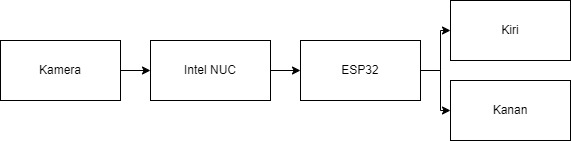
\includegraphics[scale=0.6]{gambar/hardware.jpg}

  % Ubah dengan keterangan gambar yang diinginkan
  \caption{Blok Diagram Hardware}
  \label{fig:roketluarangkasa}
\end{figure}
\subsection{Kamera}
Pada tugas akhir ini pendeteksian menggunakan data citra yang diolah untuk mendapatkan output berupa deteksi manusia yang akan dianalisa jaraknya. Kamera menjadi input utama untuk mendapatkan citra yang akan dipasangkan dalam kursi roda otonom.Posisi kamera yang digunakan harus berada pada posisi yang dapat menangkap citra manusia dengan jelas. Adapun kamera yang digunakan adalah kamera Logitech C920. 

Kamera Logitech C920 dilengkapi dengan lensa kaca Carl Zeiss dan sensor Gambar Full HD 1080p. Kamera ini juga mendukung video call dalam resolusi 720p yang berkualitas tinggi. Fitur autofocus otomatisnya memastikan bahwa Gambar tetap fokus bahkan ketika pengguna bergerak. Logitech C920 juga dilengkapi dengan dua mikrofon stereo yang dapat merespons suara dengan jelas dan natural, menghasilkan pengalaman audio yang memuaskan tanpa perlu penggunaan mikrofon eksternal. Dengan kombinasi fitur dan spesifikasi ini, Logitech C920 sudah lebih dari cukup untuk digunakan sebagai kamera untuk mendeteksi obstacle  yang hendak dideteksi.

\subsection{Intel NUC}
Intel NUC digunakan sebagai komputer pusat dalam kursi roda otonom untuk memproses citra dari kamera dan menjalankan algoritma deteksi objek. Data yang dihasilkan dari deteksi digunakan untuk mengambil keputusan navigasi. Misalnya, menghindari hambatan dan menentukan arah gerak. Perintah tersebut kemudian dikirim ke ESP32 yang mengontrol mekanisme penggerak kursi roda.

Penggunaan Intel NUC tidak langsung dapat menjalankan sistem yang dibuat, melainkan perlu diinstal library agar dapat menjalankan sistem yang telah dibuat.

\begin{lstlisting}
pip install opencv-python
pip install ultralytics
pip install mediapipe

\end{lstlisting}
opencv-python digunakan untuk menangkap dan memproses citra dari kamera. Ultralytics digunakan untuk menjalankan deteksi objek menggunakan model YOLOv8. Mediapipe digunakan untuk menampilkan landmark pada manusia
\subsection{ESP32}
Untuk dapat menggerakkan kursi roda maka perlu mengirimkan perintah ke kontroler kursi roda. ESP32 menjadi akan menerima input perintah dasar untuk menggerakkan kursi roda, seperti maju, kanan, kiri. Perintah ini kemudian akan digabungkan dengan kecepatan maksimal menjadi satu command atau paket data seperti ”Arah”. Berikut merupakan tabel kode instruksi kursi roda berdasarkan hasil deteksi \parencite{ekatama2024perancangan}

% Contoh pembuatan tabel
\begin{longtable}{|c|c|}
    \caption{Kode instruksi dari hasil klasifikasi}
    \label{tbl:kode-instruksi}\\
        \hline
        Klasifikasi Pose & Kode Instruksi \\ \hline
        \endfirsthead
        %
        \endhead
        %
        Kiri             & A              \\ \hline
        Maju             & B              \\ \hline
        Stop             & C              \\ \hline
        Mundur           & D              \\ \hline
        Kanan            & E              \\ \hline
\end{longtable}


Setelah variabel tersebut dimasukkan maka akan dikirim secara nirkabel. Dalam tugas akhir ini menggunakan wifi dengan ssid Haris-Acess-Point setelah terkoneksi.

Paket data yang telah dikirimkan melalui NUC akan diterima oleh ESP32 menggunakan WiFi. Saat diterima oleh ESP32, data tersebut akan menjalani serangkaian proses yang melibatkan pemecahan paket data dan penyesuaian sesuai dengan variabel yang telah ditentukan sebelumnya. Pemecahan paket data ini memungkinkan ESP32 untuk mendekomposisi informasi yang terkandung dalam setiap paket dan memastikan bahwa setiap variabel terpisah dengan akurat. Dengan demikian proses ini akan mengorganisir dan menyusun kembali informasi serta memastikan bahwa setiap variabel telah benar sesuai dengan nama variabel dan tipe data yang disediakan.

\subsection{Skematik Alat}

\begin{figure}[H]
  \centering

  % Ubah dengan nama file gambar dan ukuran yang akan digunakan
  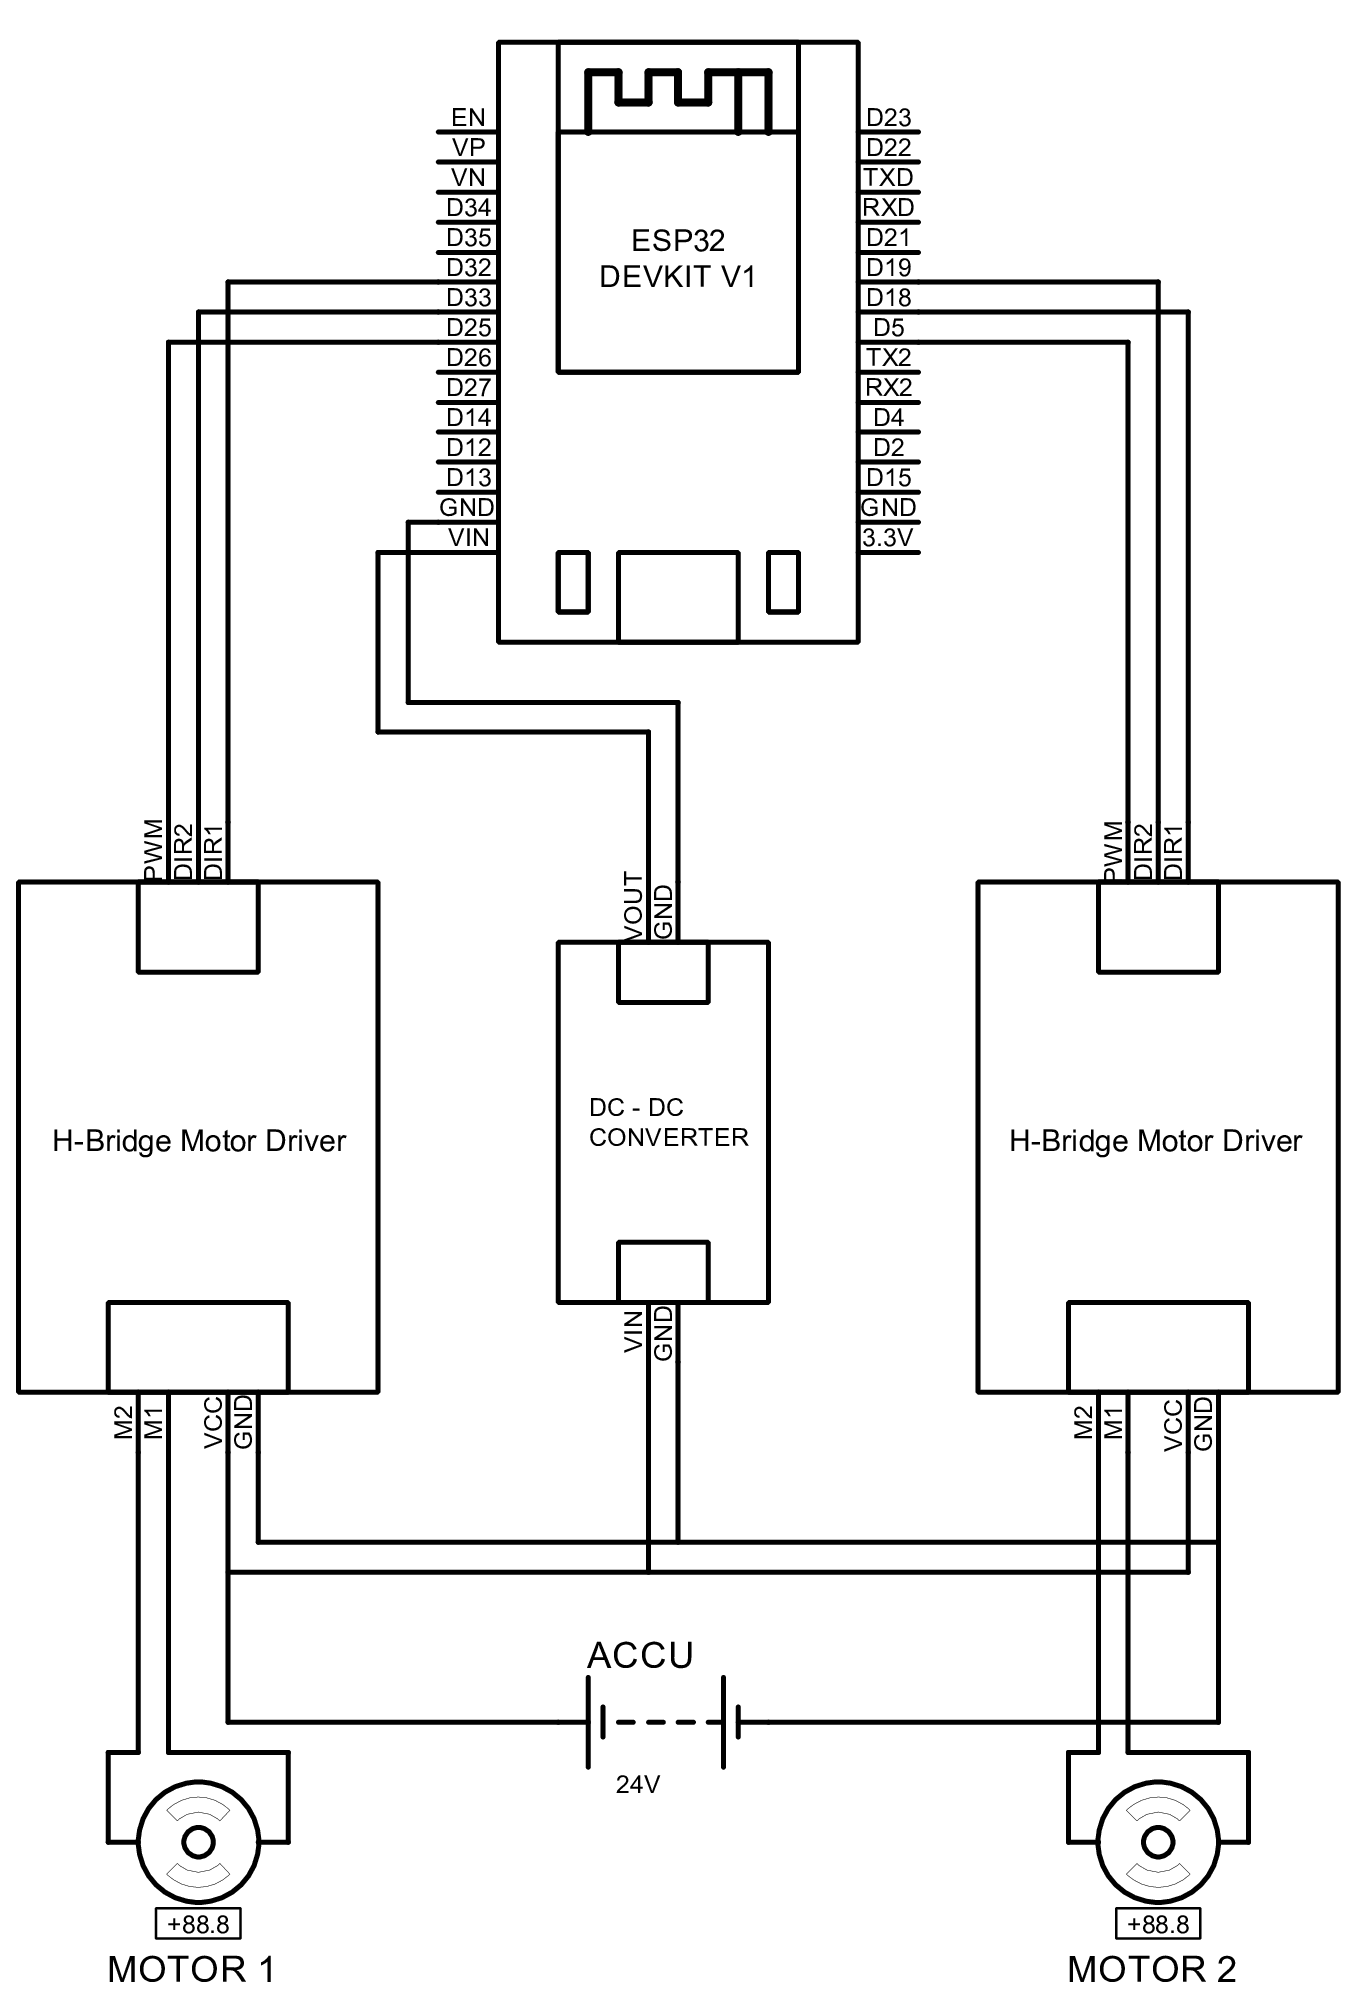
\includegraphics[scale=0.3]{gambar/Schematics.png}

  % Ubah dengan keterangan gambar yang diinginkan
  \caption{Skematik kontrol motor kursi roda}
  \label{fig:roketluarangkasa}
\end{figure}

Gambar menampilkan skema detail dari perangkat yang dibahas. Sistem ini menggunakan kamera yang terhubung ke NUC, yang berfungsi sebagai perangkat utama untuk pengambilan gambar objek. Ketika kamera berhasil menangkap gambar objek, data citra tersebut kemudian diproses oleh Laptop atau Jetson Nano. Di dalam sistem, terdapat model klasifikasi yang telah diprogram untuk menganalisis data citra ini secara detail. Hasil analisis ini sangat penting, sebab menjadi dasar dalam pembuatan kode instruksi yang akan dieksekusi oleh sistem.

Kode instruksi yang dihasilkan kemudian diintegrasikan dengan parameter kecepatan maksimal yang telah ditetapkan oleh pengguna. Integrasi antara kode instruksi tersebut kemudian dikemas dalam bentuk paket data yang digunakan untuk mengatur dan mengendalikan pergerakan kursi roda. Paket data ini selanjutnya ditransmisikan secara nirkabel, menggunakan teknologi WiFi, menuju modul ESP32 Devkit V1.

ESP32 memegang peranan kunci dalam mekanisme pengendalian motor kursi roda, berfungsi sebagai pusat pengendalian yang menerima paket data dari pengguna melalui koneksi nirkabel. Setelah menerima paket, ESP32 akan menguraikan paket data tersebut untuk menyesuaikan dengan variabel-variabel yang telah ditentukan. Proses dekripsi ini menghasilkan dua variabel utama yang akan diproses lebih lanjut oleh ESP32 untuk pengoperasian kursi roda.

Variabel utama pertama adalah variabel arah, yang memainkan peran kritis dalam menentukan arah gerakan motor-motor pada kursi roda, memastikan bahwa gerakan motor selaras dengan arah yang dikehendaki berdasarkan data yang telah dianalisis dan diterima, sehingga pergerakan kursi roda dapat dikontrol dengan aman dan efisien.\parencite{ekatama2024perancangan}


\section{Software}
Perancangan software dilakukan sesuai dengan alur yang akan dideskripsikan pada subbab ini. Perangangan ini akan dipresentasikan dengan blok diagram alur yang telah merepresentasikan alur perancangan software ini. Gambar blok diagram alur akan ditampilkan sebagai berikut :

\begin{figure}[H]
    \centering
    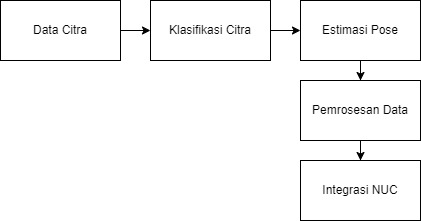
\includegraphics[scale = 0.6]{gambar/DIagram p.jpg}
    \caption{Diagram Blok Software}
    \label{fig:enter-label}
\end{figure}

\subsection{Pengumpulan Dataset citra
  \label{sec:Dataset Citra}}
Dalam pengembangan Tugas Akhir ini akan digunakan dataset citra berupa gambar, Dimana objek yang akan dideteksi pada gambar tersebut ialah Manusia yang fungsinya dalam tugas ini sebagai obstacle yang akan dihindari. citra manusia tersebut diambil melalui setiap frame citra pada video yang didapatkan menggunakan kamera webcam yang terhubung dengan komputer. Kemudian setiap citra yang didapatkan nantinya akan diproses untuk menentukan apakah terdapat manusia atau tidak pada citra tersebut. Dalam pendeteksian, nantinya proses ini terjadi secara real-time guna mendapatkan keseluruhan citra yang dibutuhkan untuk mengenali manusia atau tidak pada citra secara terus-menerus

\begin{figure}[H]
  \centering
  % Ubah dengan nama file gambar dan ukuran yang akan digunakan
  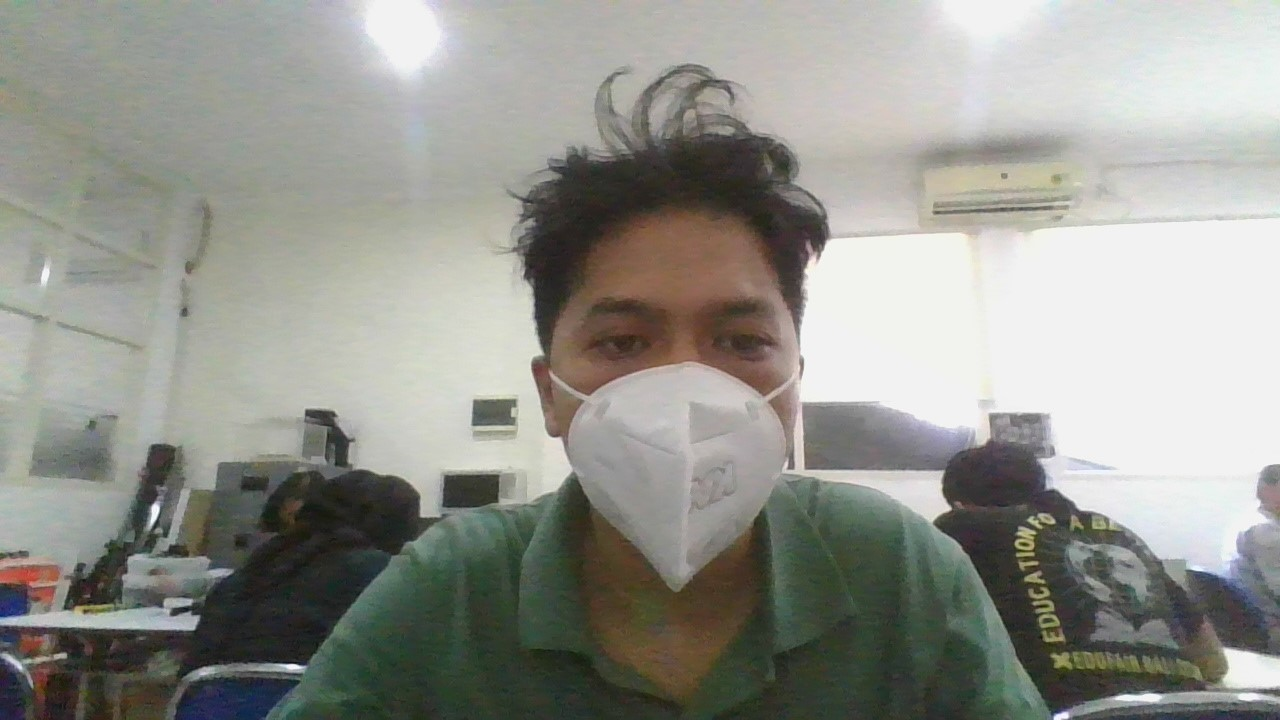
\includegraphics[scale=0.3]{gambar/WIN_20240319_17_11_26_Pro.jpg}
  % Ubah dengan keterangan gambar yang diinginkan
  \caption{Contoh Hasil data dari Citra.}
  \label{fig:Hasil Data dari Citra}
\end{figure}

Dengan menggunakan perangkat kamera yang terhubung dengan komputer, perangkat akan menghubungkan interaksi antara pengguna dengan komputer untuk mendapatkan frame citra pada video agar nantinya dapat diproses. Gambar 3.2 merupakan contoh hasil dari data citra yang didapatkan melalui perangkat kamera pada komputer. Dalam hal ini, karena yang ingin dikenali adalah manusia, maka citra gambar citra yang didapatkan harus memiliki objek manusia didalamnya.

\subsection{Labeling Menggunakan Roboflow}
Dataset citra yang sudah didapatkan selanjutnya akan melalui proses labeling dan augmentasi. Dimana Roboflow memiliki tools yang mumpuni dalam melakukan labeling. Dimana terdapat beberapa proses yang akan dilakukan yaitu, import dataset, pelabelan dataset dan augmentasi dataset

\begin{figure}[H]
  \centering
  % Ubah dengan nama file gambar dan ukuran yang akan digunakan
  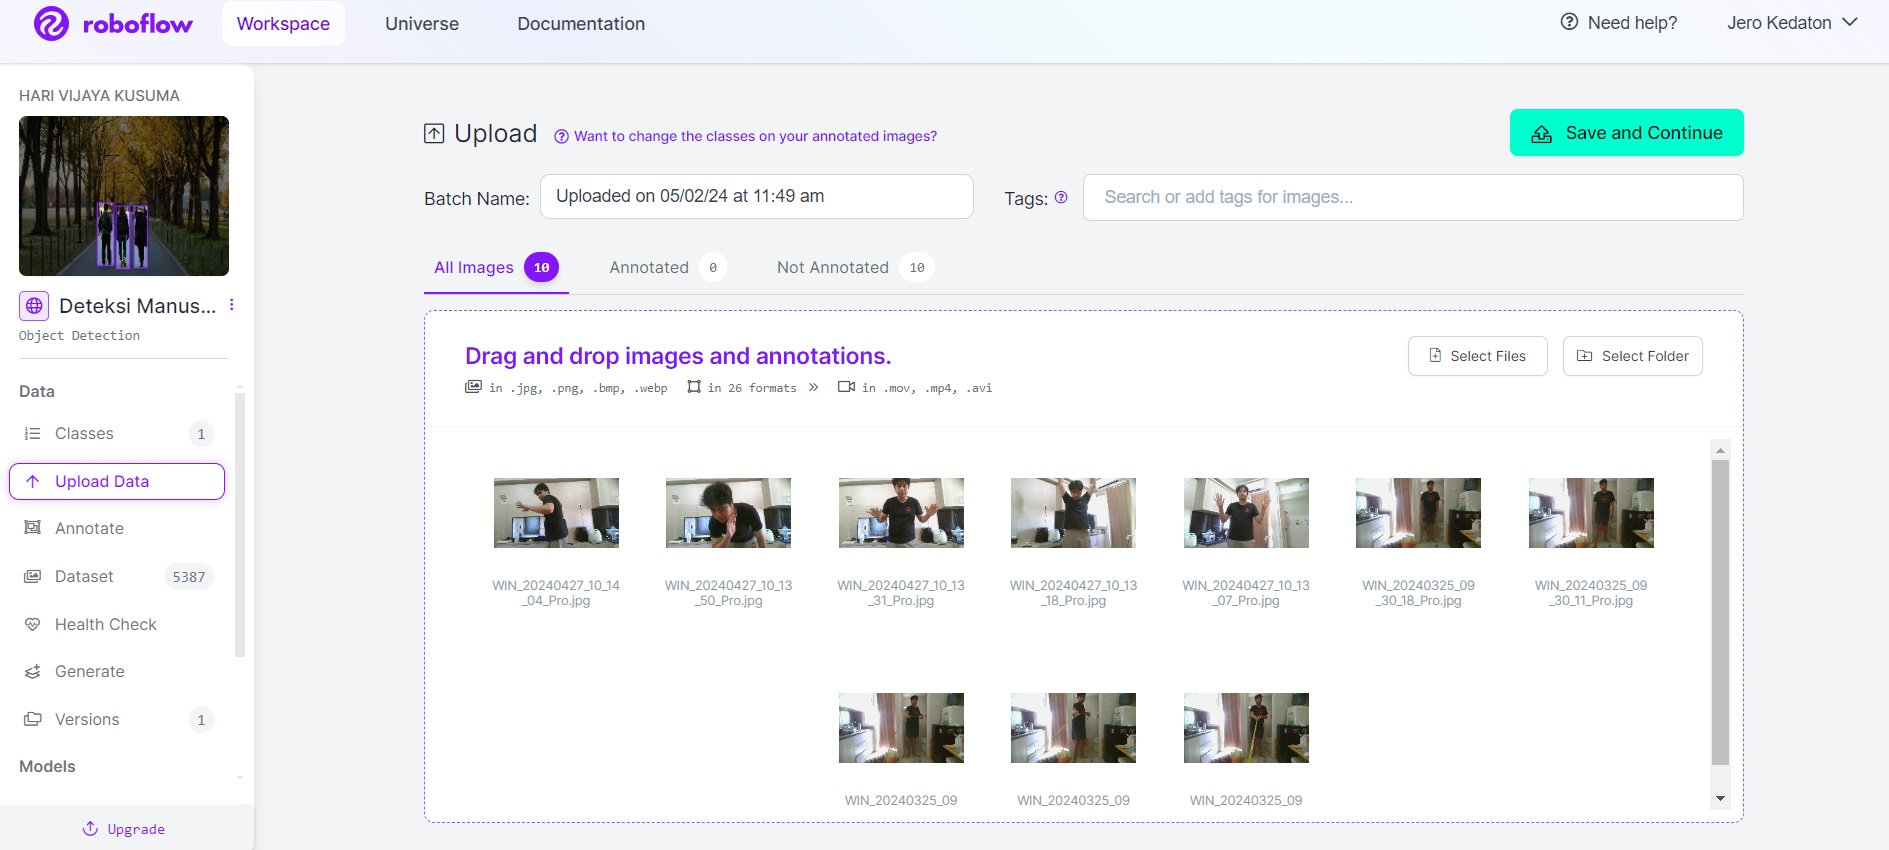
\includegraphics[scale=0.3]{gambar/roboflow upload.jpg}
  % Ubah dengan keterangan gambar yang diinginkan
  \caption{Contoh upload dataset ke roboflow.}
  \label{fig:Mengupload dataset ke roboflow}
\end{figure}

Dataset yang diupload haruslah mencakup beberapa skenario dan mencakup berbagai ukuran Setelah itu melakukan Praproses dataset dengan anotasi, yaitu mengubah ukuran Gambar, menormalkan nilai piksel, dan membaginya menjadi set training, validasi, dan test. Lalu menambah data dengan teknik seperti rotasi, penskalaan, atau membalik untuk meningkatkan keragaman sampel pelatihan.
\begin{figure}[H]
  \centering
  % Ubah dengan nama file gambar dan ukuran yang akan digunakan
  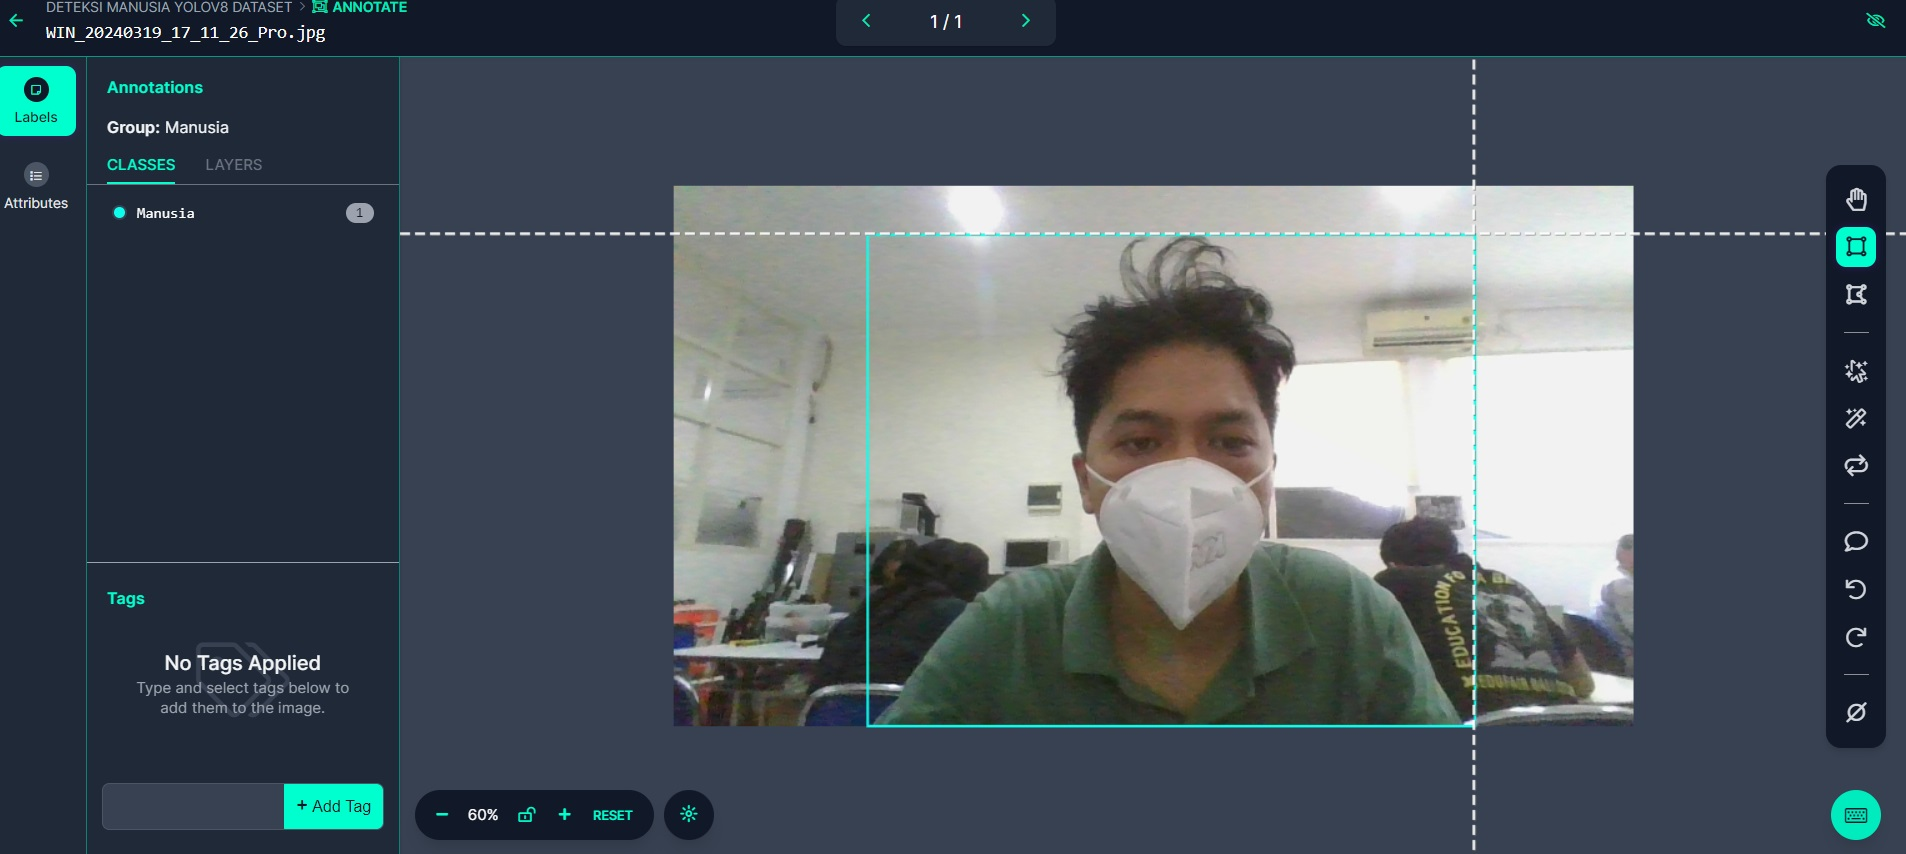
\includegraphics[scale=0.3]{gambar/roboflow anotasi.jpg}
  % Ubah dengan keterangan gambar yang diinginkan
  \caption{Contoh anotasi dataset ke roboflow.}
  \label{fig:Mengupload dataset ke roboflow}
\end{figure}

Dalam proses anotasi penamaan class yang digunakan haruslah sesuai dengan objek yang akan dideteksi. Dalam konteks tugas akhir kali ini obstacle yang dimaksud adalah manusia, maka penamaan class adalah manusia. Selain itu dalam proses anotasi harus diperhatikan posisi objek yang akan dianotasi harus jelas agar tidak ada kesalahan model dalam mendeteksi.

\begin{figure}[H]
  \centering
  % Ubah dengan nama file gambar dan ukuran yang akan digunakan
  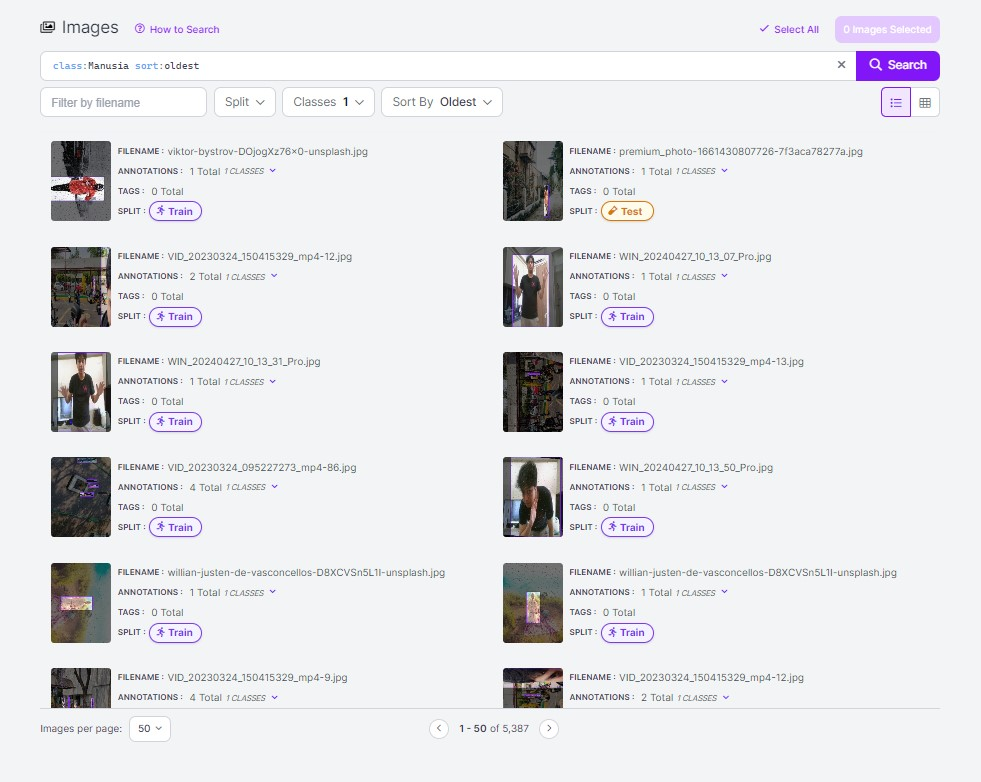
\includegraphics[scale=0.4]{gambar/roboflow Dataset.jpg}
  % Ubah dengan keterangan gambar yang diinginkan
  \caption{Contoh Dataset.}
  \label{fig:Mengupload dataset ke roboflow}
\end{figure}

Setelah seluruh Gambar yang dipilih telah dianotasi, terdapat opsi membuat datasets dan Pemilihan Gambar yang dikelompokkan dari grup batch dataset tesebut diunggah. Pengguna dapat melakukan kombinasi dan Pemilihan secara mendetil tentang Gambar spesifik apa yang dibutuhkan dalam proses pembuatan model sehingga bisa merepresentasikan hasil deteksi objek yang hendak dilakukan. Jika Gambar yang telah
dianotasi telah memenuhi kriteria yang ditetapkan, maka dibuatlah versi baru dataset dengan menekan tombol create new version berwarna biru. Kemudian pengguna dapat memilih Gambar dan mengatur konfigurasi split pada dataset, praproses dataset, serta augmentasi dataset. Berikut tampilan dari Datasets yang siap untuk dibuat yang diGambarkan pada Gambar Diatas.

Selain itu juga terdapat pula fitur preprocesssing datasets yang berasal dari roboflow dimana berguna untuk menstandarkan format Gambar (misalnya, semua Gambar berukuran sama). Langkah ini penting untuk memastikan kumpulan data Anda konsisten sebelum melatih model. Berikut fitur tesebut.

\begin{itemize}
    \item Auto - Orient
    \item Rezise
    \item Grayscale
    \item Auto Adjust Contrast
    \item Isolate Objects
    \item Static Crop
    \item Tile
    \item Modify Classes
    \item Filter Null
\end{itemize}

Adapula fitur Augmentasi data yaitu langkah di mana augmentasi diterapkan pada Gambar yang ada di kumpulan data Anda. Proses ini dapat membantu meningkatkan kemampuan model untuk menggeneralisasi sehingga bekerja lebih efektif pada Gambar yang tidak terlihat. Pada awal proses training tidak digunakan proses augmentasi guna mengevaluasi kualitas datasets yang murni yaitu belum mengalami Augmentasi. Jika augmentasi ditambahkan dan dataset tidak berkinerja sebaik yang diharapkan, maka tidak akan ada dasar untuk membandingkan kinerja model. 

\begin{figure}[H]
  \centering
  % Ubah dengan nama file gambar dan ukuran yang akan digunakan
  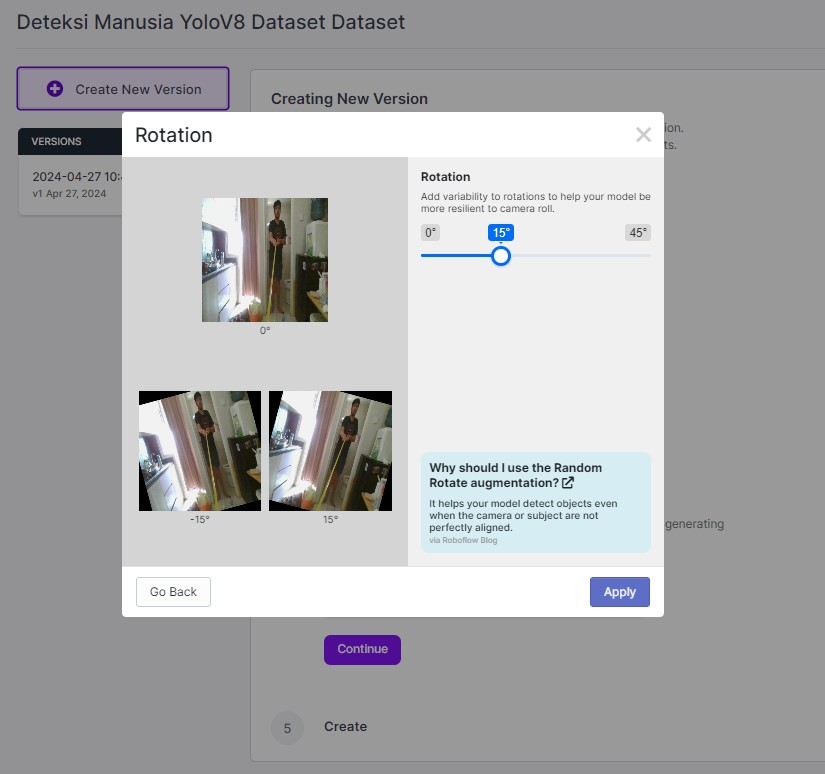
\includegraphics[scale=0.4]{gambar/roboflow augmentasi.jpg}
  % Ubah dengan keterangan gambar yang diinginkan
  \caption{Contoh Augmentasi Dataset.}
  \label{fig:Mengaugmentasi dataset ke roboflow}
\end{figure}

Jika performa model tidak baik tanpa augmentasi, hal yang perlu dilakukan yaitu menyelidiki keseimbangan kelas, representasi data, dan ukuran kumpulan data. Jika terdapat kumpulan data yang modelnya telah berhasil dilatih tanpa augmentasi, maka proses penambahan augmentasi untuk lebih membantu meningkatkan performa model dapat dilakukan.

\subsection{Object Detection YoloV8}
Deteksi Objek dilakukan dengan mendeteksi keberadaan Manusia pada citra yang didapatkan, kemudia keberadaan manusia yang terdeteksi pada citra, akan digambar bounding box pada area yang terdeteksi manusia. Dimana Bounding box yang terdeteksi tersebut akan memilki nilai nilai x dan y dalam posisi pixel pada jendela kamera yang selanjutnya dapat diambil berupa tinggi dan lebar pada pixel yang terdeteksi pada jendela web kamera. Dimana nilai nilai tersebut akan menjadi acuan dalam menentukan jarak objek relatif terhadap kamera. 

\begin{figure}[H]
  \centering
  % Ubah dengan nama file gambar dan ukuran yang akan digunakan
  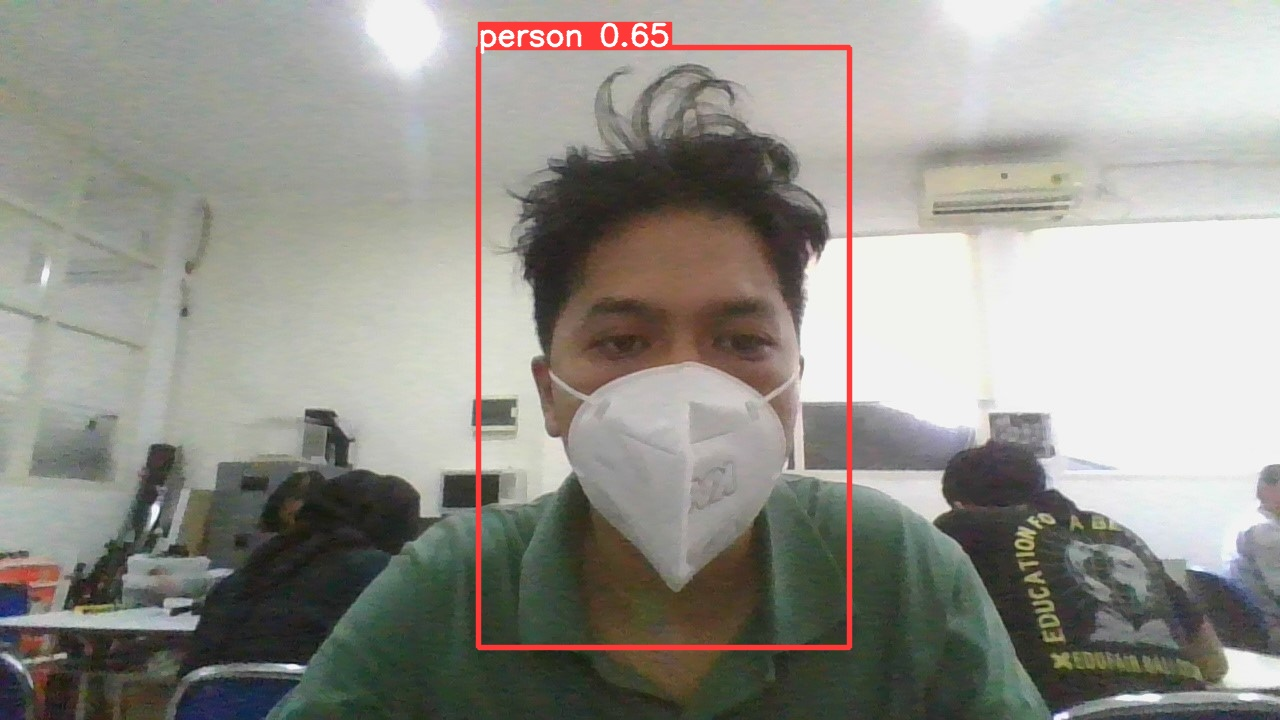
\includegraphics[scale=0.25]{gambar/Foto deteksi untuk bab 2 agung.jpg}
  % Ubah dengan keterangan gambar yang diinginkan
  \caption{Contoh Hasil Deteksi Menggunakan Model YoloV8 yang telah di train.}
  \label{fig:Mengaugmentasi dataset ke roboflow}
\end{figure}


Bounding box yang didapatkan merupakan hasil dari training yang akan dilakukan sehingga model YoloV8 dapat mengidentifikasi kelas yang diinginkan yaitu kelas Manusia. Berikut merupakan contoh gambar hasil dari identifikasi objek yang dihasilkan dari model yang telah dilakukan training. Dapat dilihat hasil deteksi menghasilkan nilai, yang merupakan nilai confidence dari model dimana nilai ini menunjukan seberapa yakin citra yang diinput merupakan bagian class yang terdeteksi.

Dalam proses training akan didapatkan beberapa nilai yang akan menjadi acuan dalam seberapa baik model dalam mendeteksi objek yang terdapat dari input citra, dimana nilai nilai tersebut akan divisualisasikan melalui confusion matrix maupun grafik yang mengindikasikan performa model dalam mendeteksi. berikut contoh gambar confusion matrix

\begin{figure}[H]
  \centering
  % Ubah dengan nama file gambar dan ukuran yang akan digunakan
  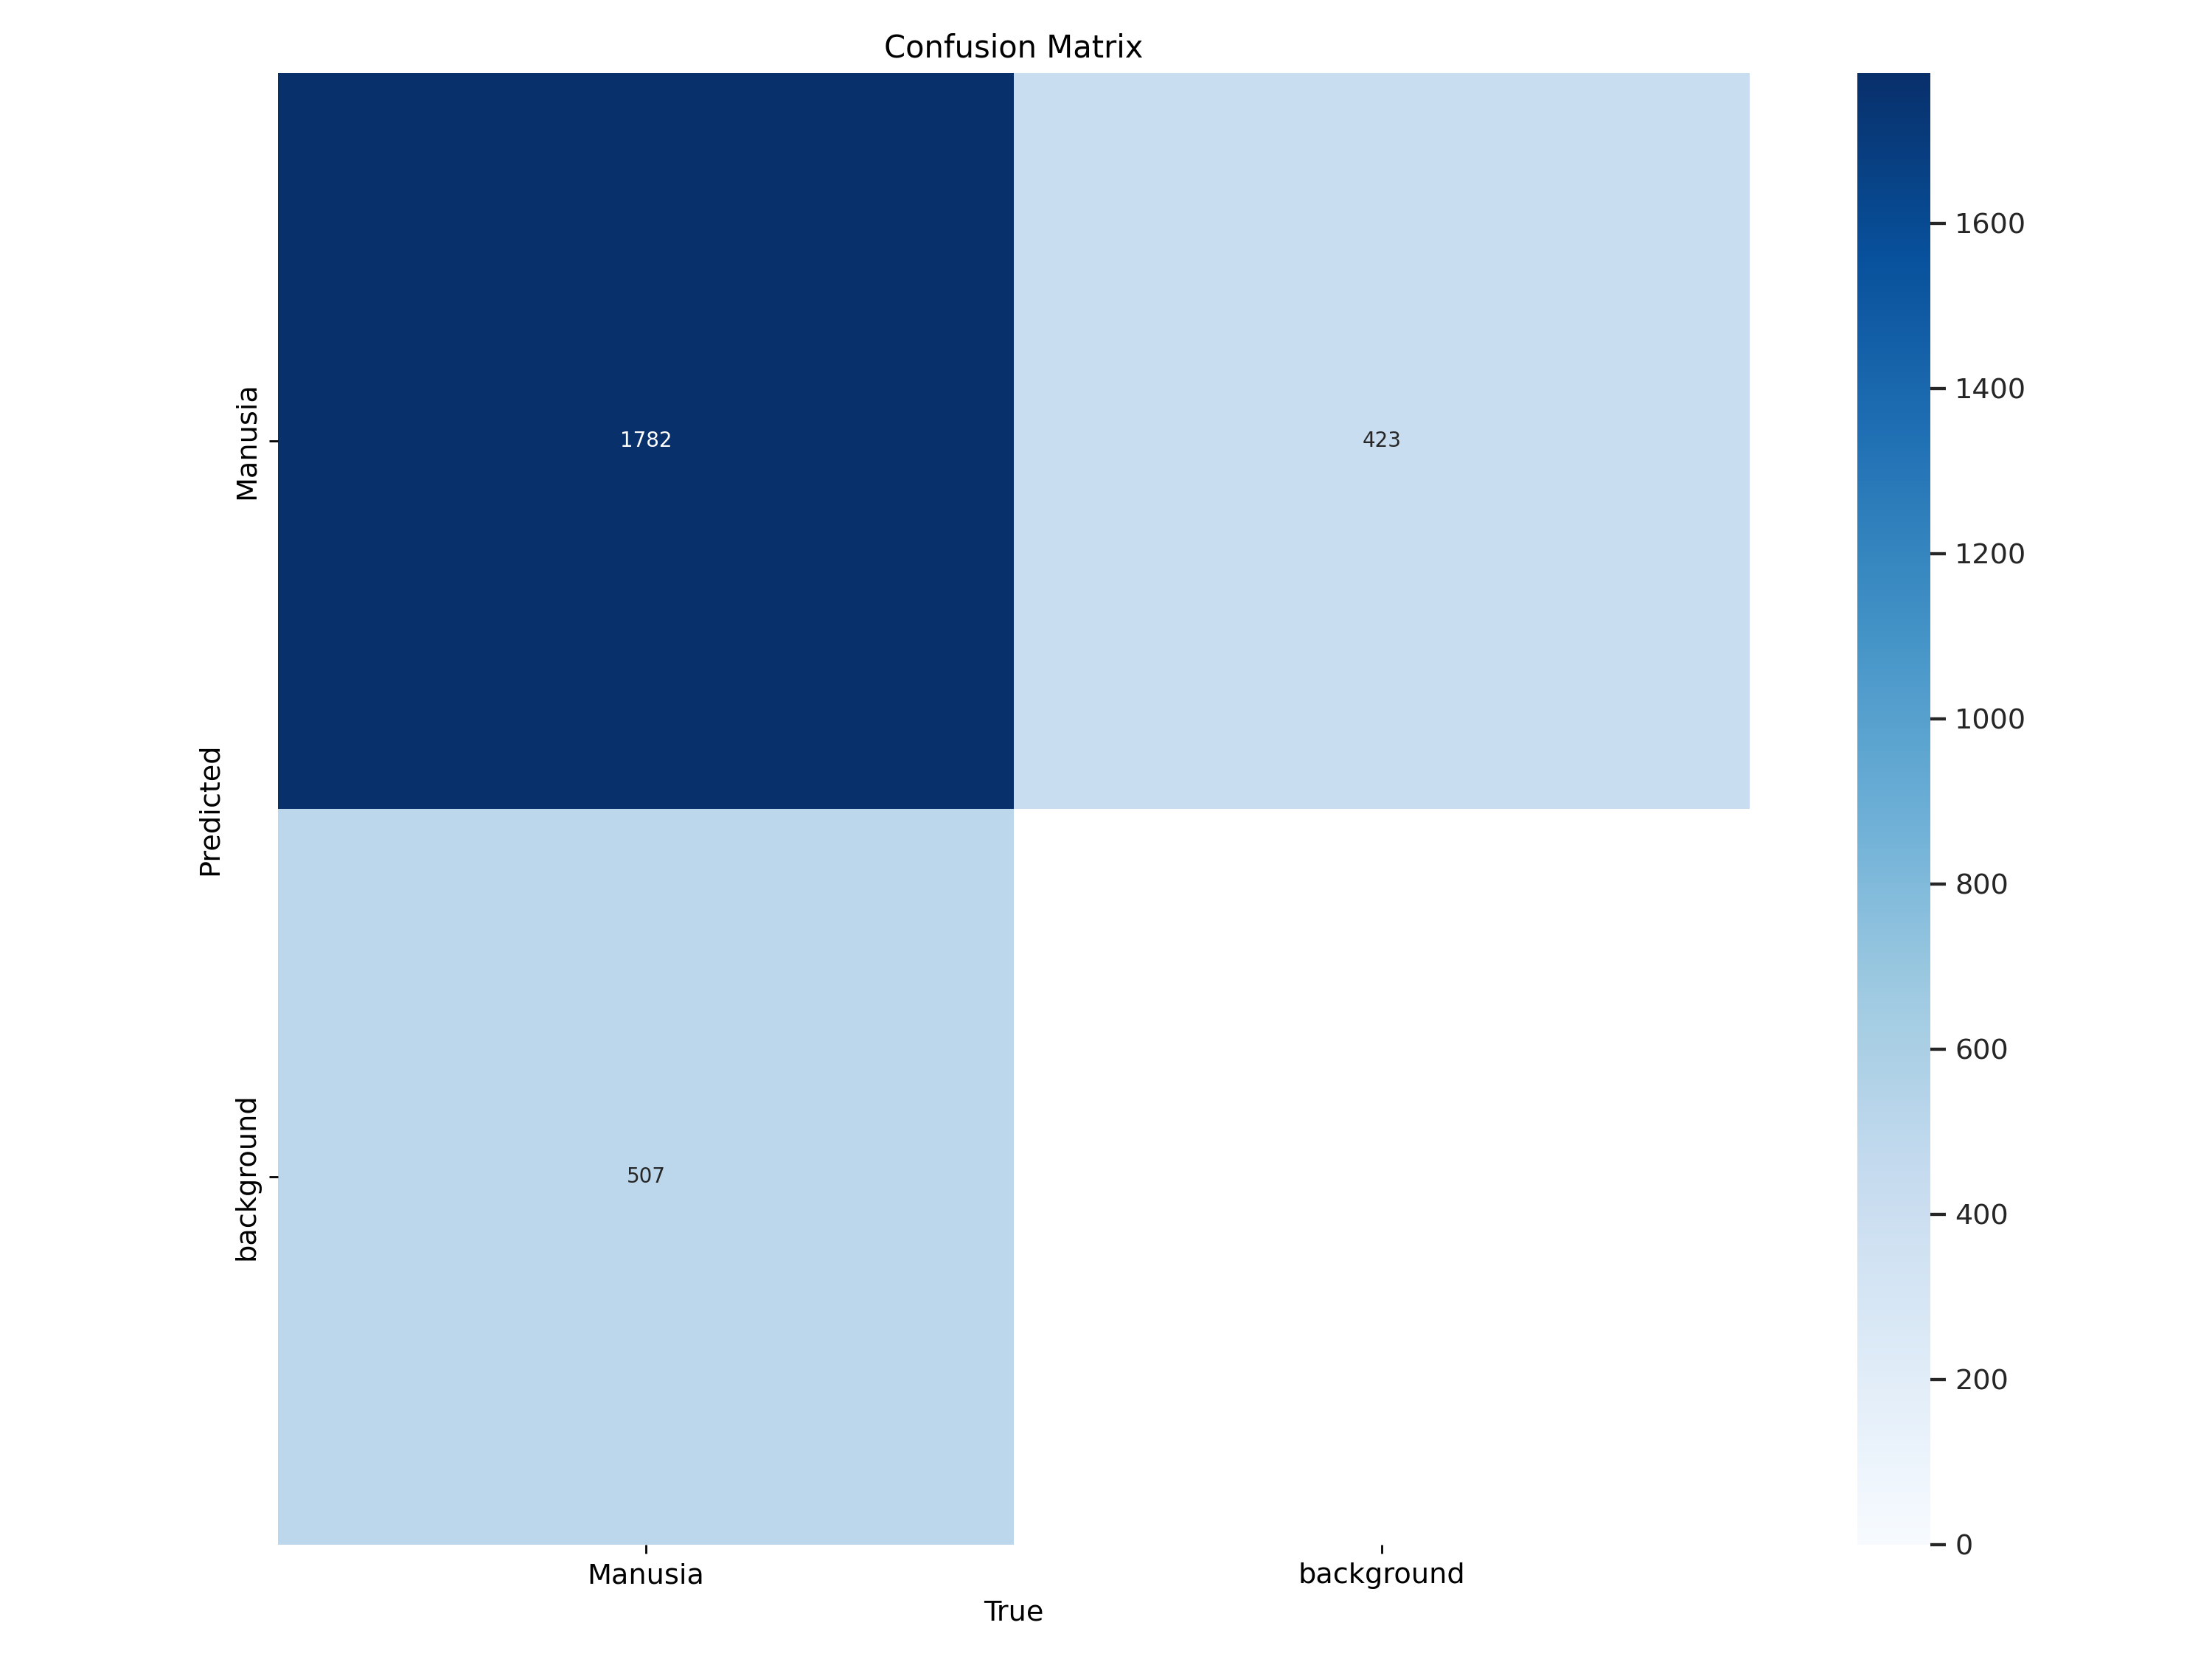
\includegraphics[scale=0.25]{gambar/download.png}
  % Ubah dengan keterangan gambar yang diinginkan
  \caption{Contoh Confusion Matrix model.}
  \label{fig:confusion matrix model}
\end{figure}

Dimana dapat dilihat pada confusion matrix dimana nilai hasil pojok kiri atas merupakan nilai true positive, sedangkan nilai pojok kanan atas merupakan false negatif, nilai pojok kiri bawah adalah false positive, dan terakhir nilai pojok kanan bawah merupakan true negative.

Selain confusion matrix juga terdapat clasification loss. Classification Loss mengukur nilai loss model dalam memprediksi klasifikasi objek yang telah ditentukan melalui proses pelabelan atau anotasi data. Sebuah nilai loss klasifikasi yang rendah menunjukkan bahwa model cenderung menjadi lebih optimal. Localization Loss, pada sisi lain, mencerminkan kinerja sistem dalam menentukan posisi suatu objek. Semakin rendah nilai loss lokalisisasi, semakin baik model yang dihasilkan. Contoh grafik tersebut dapat dilihat pada gambar berikut.

\begin{figure}[H]
  \centering
  % Ubah dengan nama file gambar dan ukuran yang akan digunakan
  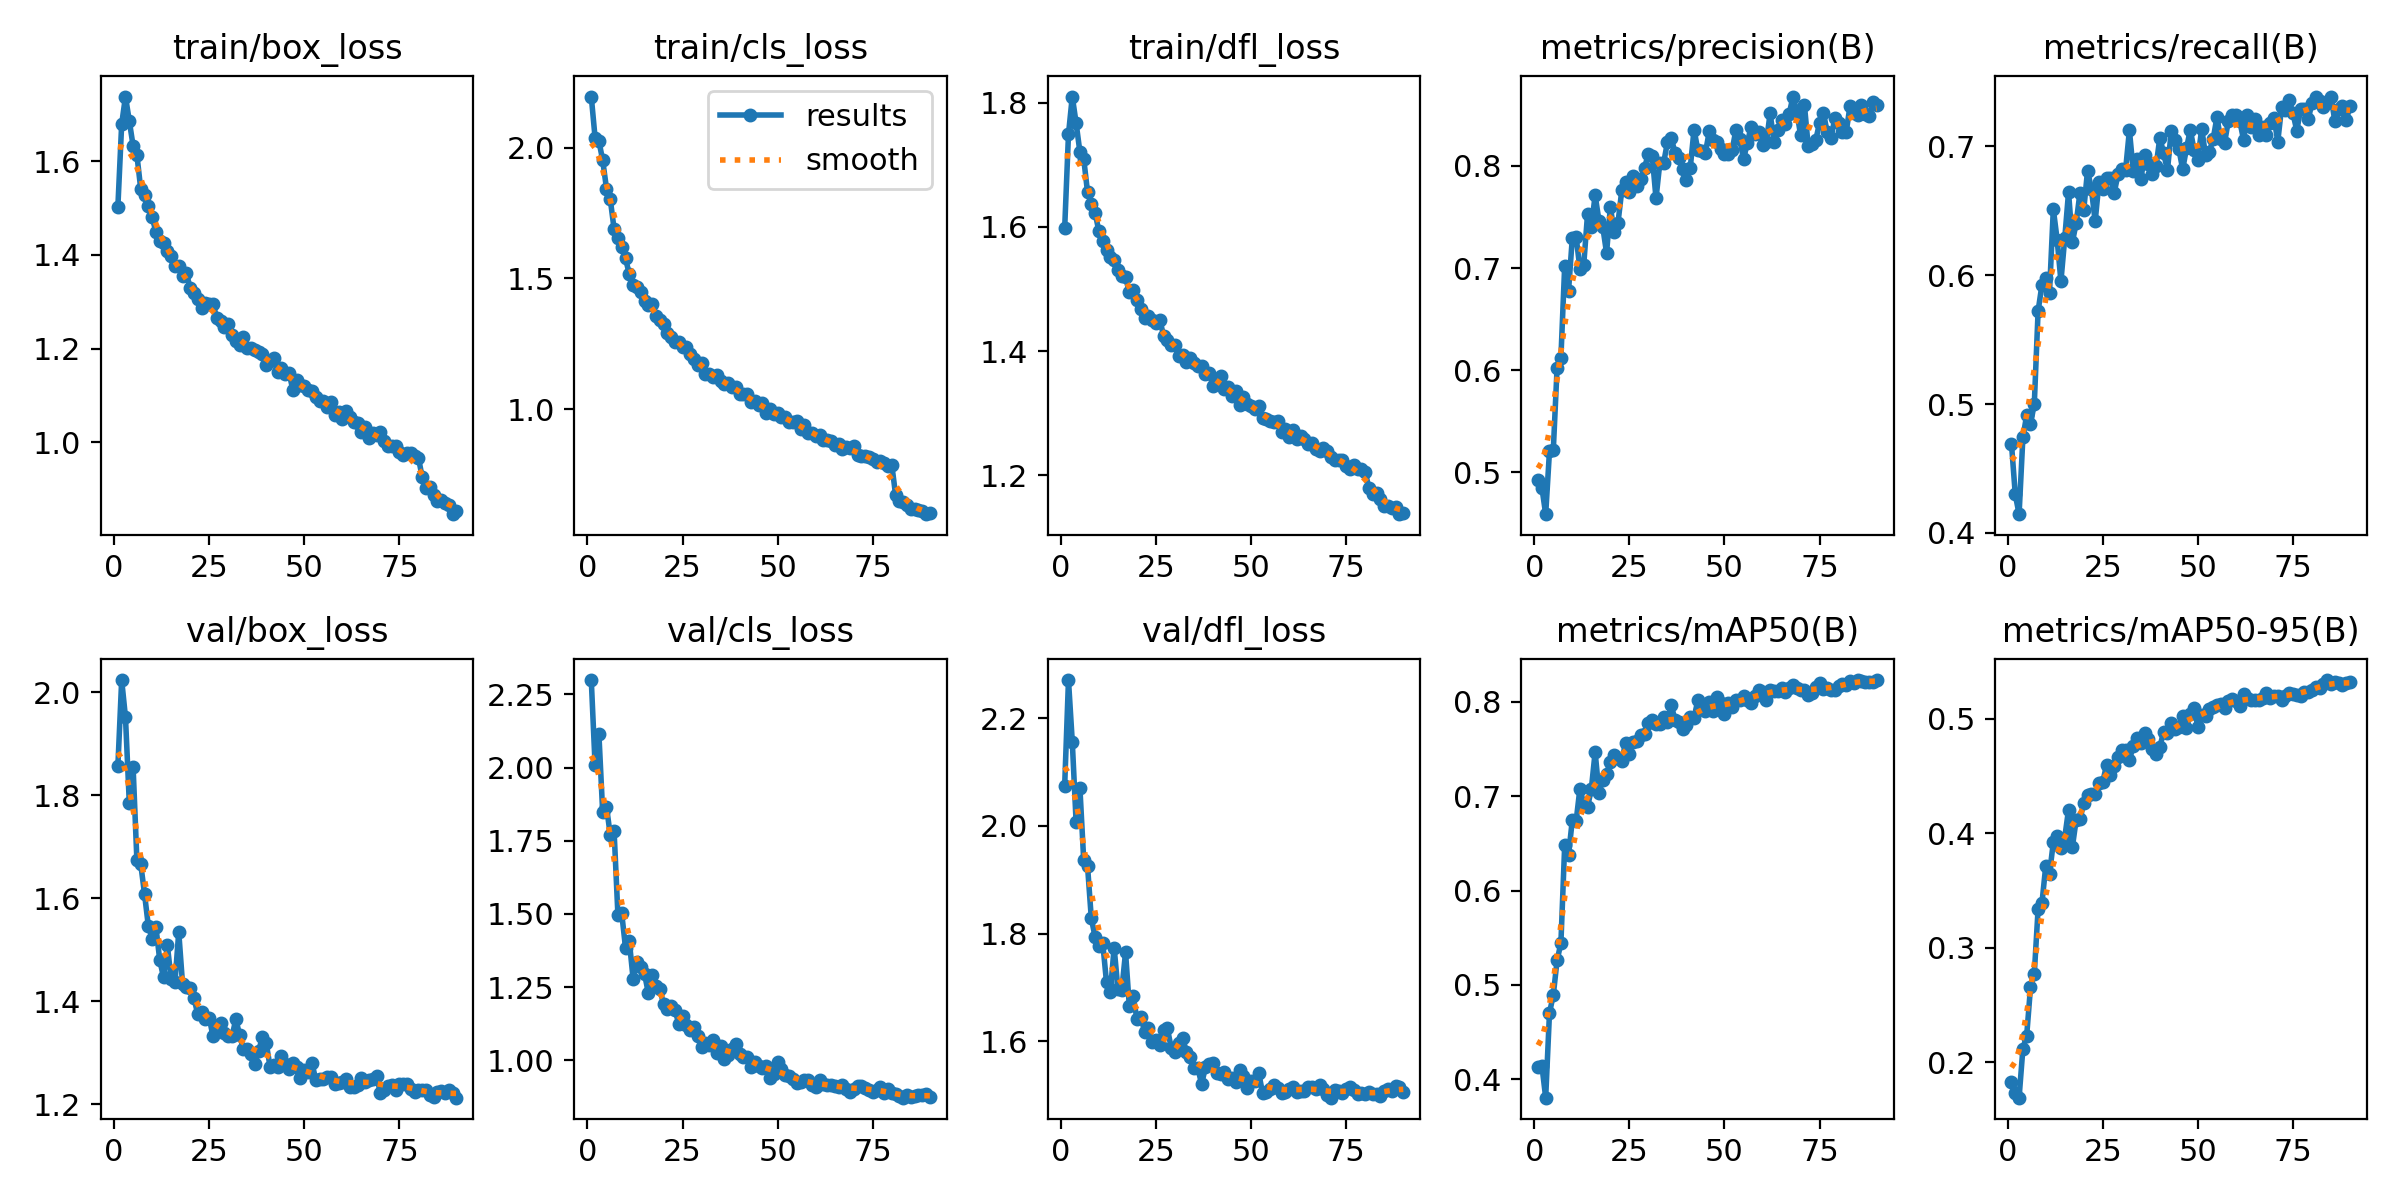
\includegraphics[scale=0.35]{gambar/map dan loss contoh.png}
  % Ubah dengan keterangan gambar yang diinginkan
  \caption{Contoh grafik loss dan mAP model.}
  \label{fig:confusion matrix model}
\end{figure}

Penurunan nilai Localization loss mencerminkan bahwa model yang telah dilatih secara pra-terlatih mampu mengidentifikasi objek dalam Gambar dan menghasilkan koordinat bounding box yang mendekati koordinat bounding box yang diannotasikan. Regularization Loss merujuk pada serangkaian teknik yang bertujuan untuk mengurangi kompleksitas model jaringan saraf selama proses pelatihan, sehingga mencegah terjadinya overfitting. Penerapan berbagai teknik regularisasi dapat membantu mengatasi masalah overfitting dalam jaringan saraf, yang pada gilirannya meningkatkan akurasi model Deep Learning saat dihadapkan pada data baru dari domain permasalahan yang sama. 

Nilai loss regularisasi mencerminkan tingkat kompleksitas model, dengan nilai yang lebih kecil mengindikasikan bahwa model memiliki kemungkinan lebih rendah untuk mengalami overfitting. Loss total mencakup seluruh proses pelatihan model dan dihitung berdasarkan tiga parameter utama, yaitu loss klasifikasi, loss lokalisisasi, dan loss regularisasi, memberikan pandangan menyeluruh terhadap proses pelatihan model. Oleh karena itu, evaluasi kinerja deteksi objek tidak hanya memperhatikan kemampuan model dalam mengklasifikasikan objek, tetapi juga dalam menentukan posisinya dengan akurasi tinggi dan menghindari overfitting yang berlebihan

Dalam penelitian ini, diperkenalkan tiga komponen utama dalam evaluasi kinerja model deteksi objek, yaitu classification loss, localization loss, dan regularization loss. Classification loss mengukur kesalahan model dalam memprediksi klasifikasi objek yang telah diidentifikasi
melalui proses pelabelan atau anotasi data. Semakin rendah nilai classification loss, semakin optimal model dianggap. Di sisi lain, localization loss mengindikasikan kemampuan sistem dalam menentukan posisi objek dalam Gambar. Penurunan nilai localization loss mencerminkan peningkatan kinerja model, terutama dalam menghasilkan koordinat bounding box yang mendekati anotasi yang sebenarnya. Regularisasi, sebagai serangkaian teknik, digunakan untuk mengurangi kompleksitas model jaringan saraf selama pelatihan, dengan tujuan menghindari overfitting. Penerapan berbagai teknik regularisasi membantu meningkatkan generalisasi model terhadap data baru. Nilai regularization loss memberikan Gambaran tentang seberapa kompleks model tersebut, dan nilai yang lebih rendah menunjukkan kemungkinan lebih kecil terjadinya overfitting.

Dapat dilihat pada bagian kanan terdapat grafik precision, dimana grafik ini menunjukkan presisi model, yaitu proporsi prediksi positif yang benar-benar positif. Grafik yang menunjukkan peningkatan secara bertahap menunjukkan bahwa model semakin jarang membuat prediksi positif yang salah. peningkatan ini juga dialami oleh grafik recall yang mana grafik Recall ini mengukur proporsi positif aktual yang berhasil dideteksi oleh model. Grafik dengan peningkatan menunjukkan bahwa model menjadi lebih baik dalam mendeteksi semua kasus positif yang ada. Selanjutnya terdapat grafik mAP (\emph{mean Average Precision}) pada threshold IoU (Intersection over Union) 50\% adalah metrik yang menilai secara keseluruhan kinerja model dalam mendeteksi objek dengan keakuratan yang diberikan. Nilai yang lebih tinggi menunjukkan performa yang lebih baik. dan terakhir mAP50-95 Grafik ini mirip dengan mAP50 tetapi dihitung sebagai rata-rata dari IoU yang berkisar dari 50\% hingga 95\%. Ini adalah metrik yang lebih ketat dan menunjukkan kinerja model secara lebih rinci dalam berbagai tingkat ketat deteksi.

\subsection{Estimasi Pose MediaPipe}
Deteksi pose dilakukan dengan menggunakan Python dengan library OpenCV dan frame-work MediaPipe menggunakan fungsi pose detection saat objek manusia terdeteksi dalam frame citra . Framework MediaPipe digunakan untuk mendapatkan landmark pada tubuh peraga, lalu landmark yang relevan akan digambarkan garis berbentuk kerangka yang sesuai dengan pose tubuh peraga. Dalam penelitian ini, landmark yang relevan yaitu keypoint siku atas hingga lengan bawah dan bahu kanan dan kiri. Titik keypoint yang digunakan pada estimasi pose dapat dilihat pada Tabel dibawah ini.

\begin{longtable}{|c|c|}
  \caption{Tabel Keypoint yang digunakan}
  \label{tb:EnergiKecepatan}                                   \\
  \hline
  \rowcolor[HTML]{C0C0C0}
  \textbf{Nomor Keypoint} & \textbf{Nama Keypoint}  \\
  \hline
  11            & RIGHT\_SHOULDER        \\
  12            & LEFT\_SHOULDER         \\
  14            & RIGHT\_ELBOW           \\
  16            & RIGHT\_WRIST           \\
  \hline
\end{longtable}

Dari titik landmark yang didapat akan diambil jarak terhadap pixelnya dimana nilai pixel yang didapatkan akan menjadi acuan dalam perhitungan yang akan digunakan untuk menghindari obstacle. berikut contoh landmark pada data citra.

\begin{figure}[H]
  \centering
  % Ubah dengan nama file gambar dan ukuran yang akan digunakan
  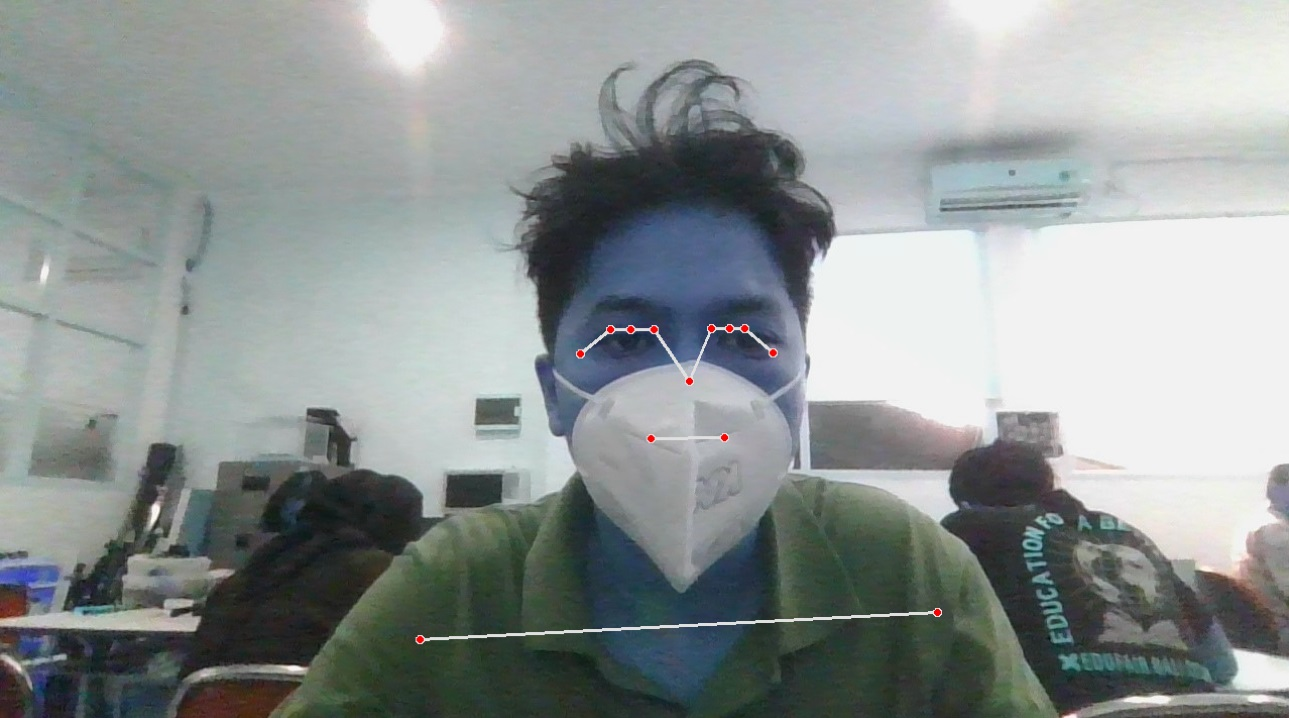
\includegraphics[scale=0.35]{gambar/fotomediapipe.jpg}
  % Ubah dengan keterangan gambar yang diinginkan
  \caption{Contoh hasil deteksi pose.}
  \label{fig:confusion matrix model}
\end{figure}

\begin{figure}[H]
  \centering
  % Ubah dengan nama file gambar dan ukuran yang akan digunakan
  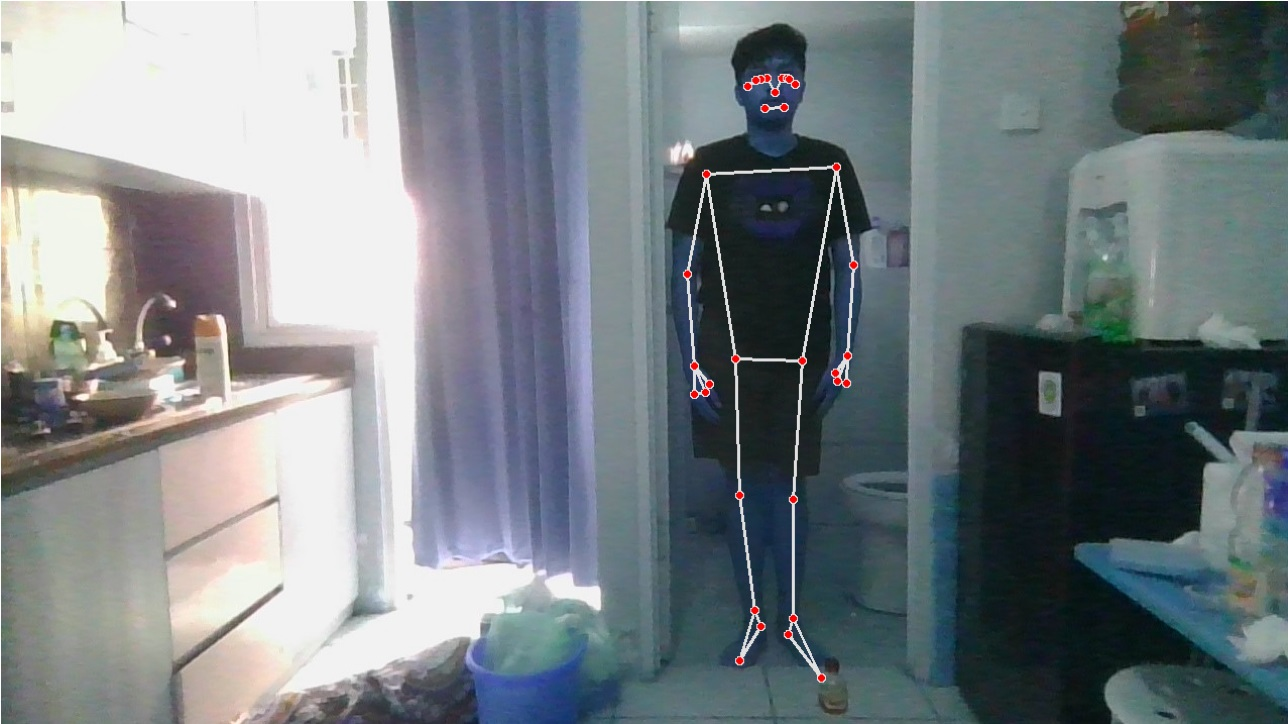
\includegraphics[scale=0.35]{gambar/fotomediapipe2.jpg}
  % Ubah dengan keterangan gambar yang diinginkan
  \caption{Contoh hasil deteksi pose seluruh tubuh.}
  \label{fig:confusion matrix model}
\end{figure}

Pengunaan landmark lengan dan bahu sebagai acuan dalam perhitungan berdasar pada visibilitas, dimana visibilitas kedua landmark ini cenderung lebih baik ketimbang landmark kaki dan kepala terutama dalam kasus penghindaran manusia. Dimana dalam jarak dekat kedua landmark ini akan lebih terlihat ketimbang landmark lainnya. Selain itu penggunaan landmark ini juga dapat menghasilkan nilai yang lebih konsisten ketimbang landmark lainnya.

\subsection{Perhitungan Rumus}

Untuk dapat menentukan jarak, pertama tama model Yolo akan digunakan untuk mendeteksi class Manusia yang akan menjadi obstacle dalam tugas akhir ini. Dari hasil deteksi yang didapat akan digambar Bounding Box penanda kelas telah terdeteksi. Dimana dalam bounding box tersebut juga akan digambar Estimasi Pose dari MediaPipe. Kedua hasil deteksi ini yaitu Bounding Box dan Pose yang dihasilkan akan digunakan untuk mendapat estimasi jarak berdasarkan rumus yang akan dijabarkan, dimana hasil dari jarak yang didapatkan akan dipetakan perpindahannya dalam grid. Dimana grid ini akan menjadi acuan dari keputusan belok yang akan diambil. berikut merupakan contoh gambar pemetaan hasil deteksi dan pengambilan keputusan belok.

\begin{figure}[H]
  \centering
  % Ubah dengan nama file gambar dan ukuran yang akan digunakan
  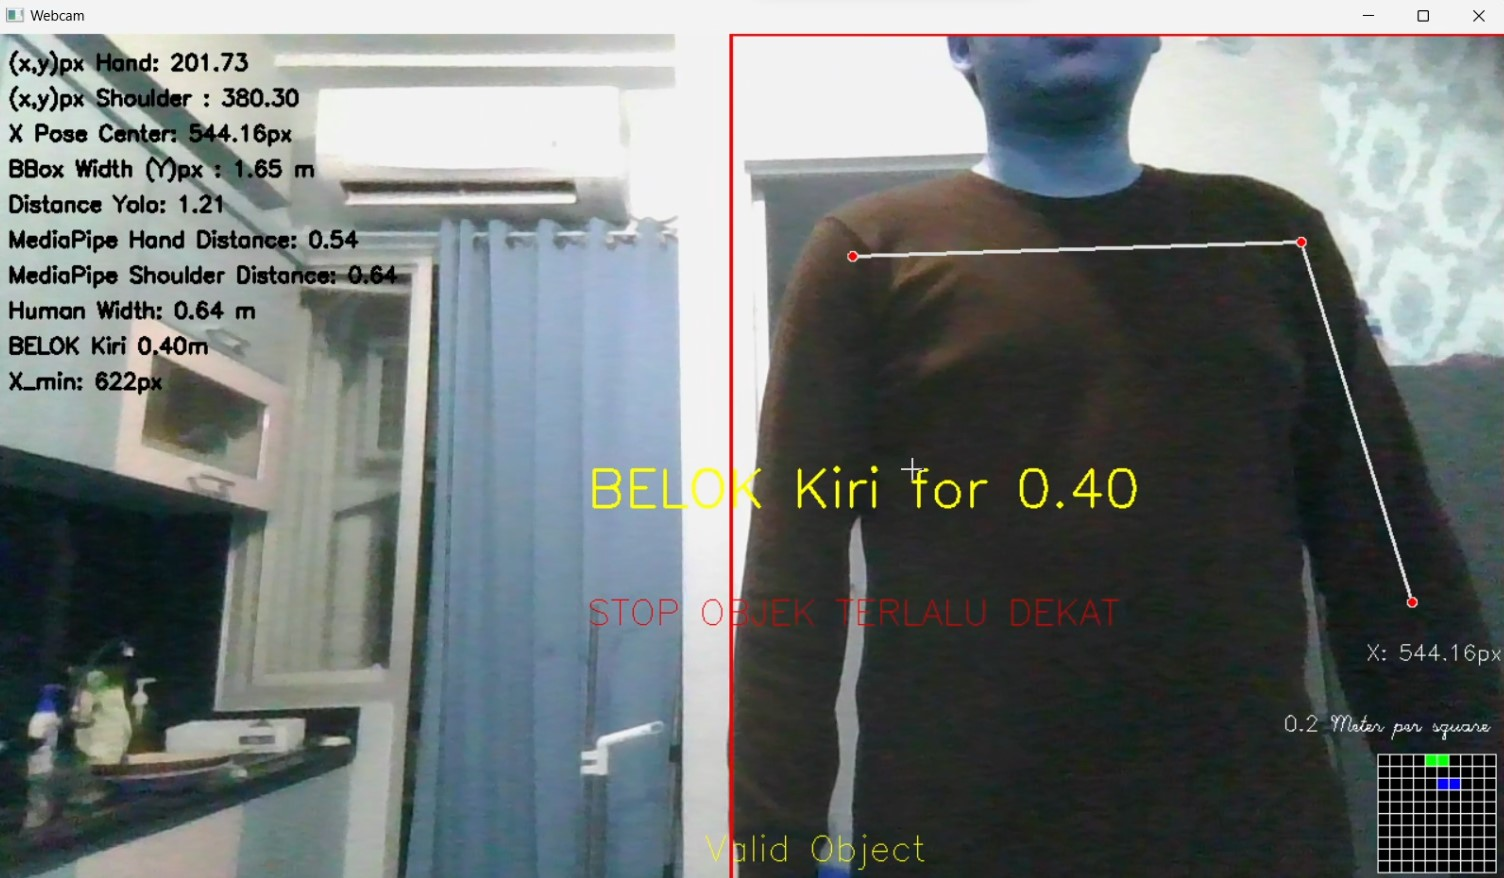
\includegraphics[scale=0.35]{gambar/belokkiri.jpg}
  % Ubah dengan keterangan gambar yang diinginkan
  \caption{Contoh Penerapan hasil perhitungan jarak dan pemetaan grid.}
  \label{fig:Penerapan hasil perhitungan jarak dan pemetaan grid}
\end{figure}

Dapat dilihat bahwa Terdapat banyak variabel pada jendela web kamera. Semua variabel tersebut memiliki peran masing masing, yang akan membantu mendapatkan nilai yang akan dipetakan dalam grid pada bagian kiri bawah.

Dalam Tugas Akhir ini terdapat beberapa variabel yang akan diukur. Variabel-variabel tersebut yaitu jarak manusia, lebar manusia, dan posisi manusia. Dimana Jarak manusia ini akan dibedakan menjadi 2 perhitungan, dimana 2 perhitungan ini berdasarkan 2 hasil deteksi yang didapatkan yaitu bounding box dan pose.

\subsubsection*{1. Perhitungan Jarak Obstacle berdasarkan Bounding Box}
Salah satu cara untuk mendapatkan jarak melalui Bounding Box adalah dengan menggunakan \emph{Focal Length Pixel}. Fokus panjang dalam piksel, atau \emph{focal length pixel}, adalah sebuah konversi dari fokus panjang lensa kamera yang biasanya diukur dalam milimeter ke dalam satuan piksel. Ini adalah konsep kunci dalam fotogrametri dan visi komputer yang digunakan untuk menghubungkan informasi visual yang diperoleh dari kamera ke ukuran fisik dalam dunia nyata.

Dalam konteks tugas akhir ini Fokus panjang dalam piksel digunakan untuk mengkonversi ukuran halangan dari unit piksel menjadi unit meter. Ini penting karena kursi roda otonom perlu memahami jarak nyata ke halangan untuk mengambil keputusan navigasi yang tepat. Dalam penggunaannya dapat dilihat dalam rumus berikut.

\begin{equation}
    focal\_length\_pixel = \left (\frac{jarak\times tinggi\_bounding\_box }{tinggi\_objek\_nyata}\right )
\end{equation}

Fokus panjang dalam piksel adalah parameter penting dalam perhitungan jarak Anda. Ini digunakan untuk mengonversi pengukuran dari ruang gambar (piksel) menjadi dimensi dunia nyata (seperti meter). Nilai ini mewakili fokus panjang lensa kamera dalam satuan piksel, yang diperoleh dari prosedur kalibrasi. 

Saat menghitung jarak ke objek dengan menggunakan tinggi dari bounding box yang terdeteksi oleh YOLO, dikombinasikan dengan tinggi nyata objek yang diketahui dan fokus panjang dalam piksel. penerapannya dapat dilihat sebagai berikut :

\begin{equation}
    jarak = \left ( \frac{focal\_length\_pixel \times tinggi\_objek\_nyata}{tinggi\_bounding\_box} \right )
\end{equation}

Di sini, tinggi\_objek\_nyata mungkin merupakan tinggi rata-rata orang atau objek lain yang diidentifikasi sebagai obstacle. Dengan menggunakan tinggi bounding box yang dideteksi oleh YOLOv8, kursi roda dapat menghitung jarak ke objek tersebut, yang sangat penting untuk menghindari benturan dan pengambilan keputusan.

\subsubsection*{2. Perhitungan Jarak Obstacle berdasarkan Pose}
Salah satu pendekatan yang baik dalam menentukan jarak dengan pose adalah menggunakan metode Jarak Euclidean. Jarak Euclidean dalam piksel adalah metode untuk mengukur jarak lurus antara dua titik dalam ruang gambar, yang biasanya diukur dalam piksel. Dalam konteks tugas akhir ini yang melibatkan kursi roda otonom dengan integrasi MediaPipe, pengukuran ini sangat penting untuk berbagai fungsi, terutama dalam analisis pose dan penilaian proporsi objek dalam citra yang dihasilkan oleh kamera. 

\begin{equation}
    {jarak\_euclidean} = \sqrt{(x_2 - x_1)^2 + (y_2 - y_1)^2} \times scale\_factor
\end{equation}

Rumus ini menghasilkan jarak antara dua titik dalam satuan yang sama dengan satuan koordinat \emph{x1,y1} dan \emph{x2,y2} Biasanya, jika koordinat-kordinat ini diukur dalam piksel, maka jarak yang dihasilkan juga akan dalam piksel.

Penambahan faktor skala ke dalam perhitungan jarak Euclidean berguna ketika perlu mengkonversi jarak dari satu unit ke unit lain, atau ketika koordinat titik disesuaikan ke skala tertentu yang tidak merefleksikan dimensi sebenarnya dalam piksel. Normalisasi Koordinat Dalam banyak aplikasi visi komputer, koordinat titik mungkin dinormalisasi ke skala [0, 1]. Di sini \emph{x1,y1} dan \emph{x2,y2} dalah proporsi dari lebar dan tinggi gambar. Untuk menghitung jarak nyata dalam piksel, perlu mendapatkan hasik kali dari rumus Euclidean dengan dimensi gambar.

Dari perhitungan diatas masih didapatkan jarak yang bernilai pixel. Dalam konteks perhitungan jarak perlu menggunakan niali standar dalam Meter agar perhitungan tersebut sesuai dengan kaidah yang berlaku pada umumnya. Agar nilai pixel tersebut dapat berubah menjadi meter maka perlu dilakukan kalibrasi menggunakan nilai K. nilai K merupakan nilai kalibrasi berdasarkan pengukuran eksperimental. rumusnya dapat dilihat sebagai berikut. 

\begin{equation}
    jarak\_meter = \left(\frac{k}{{jarak\_pixel}}\right)
\end{equation}

Nilai k menentukan seberapa besar pengaruh jarak dalam piksel terhadap jarak dalam meter. Nilai yang lebih besar atau lebih kecil akan secara langsung mempengaruhi hasil perhitungan jarak. Misalnya, nilai k yang lebih besar akan menghasilkan jarak yang lebih kecil untuk jumlah piksel yang sama. Nilai ini digunakan dalam konteks yang sangat spesifik di mana parameter tersebut menggambarkan hubungan langsung antara ukuran piksel dan jarak atau dimensi nyata, berdasarkan asumsi spesifik tentang geometri scene dan karakteristik kamera.

Nilai ini harus dikalibrasi secara akurat agar sesuai dengan karakteristik spesifik kamera dan setup yang digunakan. Kalibrasi yang tidak tepat akan menghasilkan pengukuran jarak yang tidak akurat, yang bisa berdampak pada keputusan navigasi kursi roda otonom. berikut rumus untuk pengkalibrasian nilai K:

\begin{equation}
    k ={{Jarak\_nyata\_objek}\times{Ukuran\_objek\_dalam\_piksel}}
\end{equation}

Nilai k mungkin perlu disesuaikan jika kondisi lingkungan berubah, seperti perubahan pencahayaan yang mempengaruhi visibilitas atau ketepatan deteksi landmark oleh MediaPipe.

\subsubsection{3. Perhitungan Lebar Obstacle Berdasarkan Pose}
Dalam perhitungan lebar juga menggunakan perhitungan jarak euclidean namun yang membedakan adalah konteks spesifikasi aplikasi. Dimana kedua pendekatan ini berbeda dalam aplikasi dan konteksnya. 

\begin{equation}
    {width\_pixel} = \sqrt{(x_2 - x_1)^2 + (y_2 - y_1)^2} \times {scale\_factor}
\end{equation}

Dimana sesuai dengan dijelaskan sebelumnya nilai output yang didapatkan adalah pixel dari lebar manusia. untuk memetakan lebarnya pixel ke meter maka perlulah membuat sebuah rumus konversi yang menentukan ukuran dalam pixel (yang merupakan ukuran digital dan relatif dikonversikan ke ukuran dunia nyata (meter)). sehingga rumusnya menjadi : 
\begin{equation}
    {width\_meters} = width\_pixel \times scale\_factor
\end{equation}

Dengan mengalikan lebar objek dalam piksel dengan faktor skala, hasilnya adalah lebar objek dalam meter. Rumus ini berguna, misalnya, dalam aplikasi dimana perlu untuk mengetahui dimensi fisik objek dalam dunia nyata untuk membuat keputusan atau pengukuran yang tepat.

Faktor skala adalah nilai yang mengonversi ukuran dari unit piksel ke unit meter. Nilai ini diperoleh melalui proses kalibrasi. Faktor skala menentukan berapa meter yang diwakili oleh setiap piksel dalam gambar, berdasarkan jarak kamera ke objek dan pengaturan kamera lainnya seperti fokus panjang. Selain itu perlu diketahui bahwa faktor skala yang digunakan pada rumus ini berbeda dengan rumus jarak yang sebelumnya dijabarkan. berikut rumus untuk mengkalibrasi faktor skala dalam konteks lebar objek:

\begin{equation}
    {scale\_factor} = \frac{{dimensi\_nyata\_rata-rata}}{{ukuran\_dalam\_piksel\_rata-rata}}
\end{equation}

Nilai-nilai ini dapat digunakan dalam kode untuk mengonversi ukuran dalam piksel ke ukuran nyata berdasarkan pengukuran yang telah dikalibrasi. Dan sekali lagi pastikan kalibrasi dilakukan dengan baik dan benar agar mendapatkan hasil yang akurat. 

\subsection{Visualisasi hasil deteksi dalam Grid}
Dalam tugas akhir ini, kursi roda otonom harus dapat mengetahui posisi obstacle yang akan dilaluinya. Oleh karena itu perlu dibuatnya sebuah peta yang dapat digunakan sebagai acuan kursi roda untuk mengambil tindakan berdasarkan jarak obstacle dan lebar obstacle yang akan menjadi acuan untuk menjawab permasalan, yaitu di titik mana kursi roda harus menghindar dan berhasilkah obstacle dihindari. Grid menjadi salah satu pendekatan terbaik dalam memetakan hasil deteksi, dimana penggunaan grid tidak hanya mempermudah dalam pengambilan tindakan, namun grid juga memberikan visualisasi mudah untuk dimengerti. Dimana ukuran grid juga dapat dicustom sesuai dengan kebutuhan, baik dimensi maupun tampilannya. 

Setelah perhitungan rumus diatas diimplementasikan dalam kode. Maka akan didapatkan beberapa variabel penting yang akan digunakan dalam memetakan posisi maupun ukuran obstacle dalam grid. sebelum itu berikut tampilan grid yang digunakan. 

\begin{figure}[H]
  \centering
  % Ubah dengan nama file gambar dan ukuran yang akan digunakan
  
\includegraphics[scale=0.3]{gambar/gridtanpakamera2.jpg}
  % Ubah dengan keterangan gambar yang diinginkan
  \caption{Grid 10x10.}
  \label{fig:Grid10x10}
\end{figure}

Penggunaan grid 10x10 didasari atas hasil citra dan performa model. Dimana baik bounding box maupun pose memiliki keterbatasan dimana hasil perhitungannya tidak melebihi parameter yang akan ditetapkan pada grid. Dimana parameter tersebut ialah sebagai berikut

\begin{figure}[H]
  \centering
  % Ubah dengan nama file gambar dan ukuran yang akan digunakan
  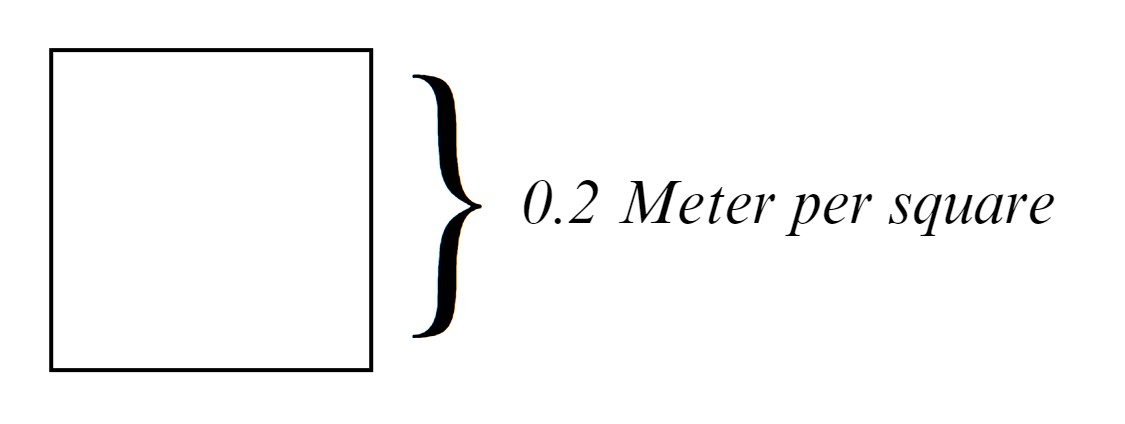
\includegraphics[scale=0.35]{gambar/02meter.jpg}
  % Ubah dengan keterangan gambar yang diinginkan
  \caption{Parameter untuk setiap kotak grid.}
  \label{fig:Parameter grid}
\end{figure}

Dapat dilihat dari gambar diatas, merupakan tetapan yang didasari dari performa diatas yang dimana setiap kotak dalam grid tersebut akan bernilai 0.2 meter baik dalam posisi vertikal maupun horizontal.

Agar dapat memetakan objek dengan baik dalam grid maka diperlukannya index untuk mengetahui posisi relatif kiri dan kanan objek terhadap kamera. Dimana untuk 10 kotak horizontal akan dibagi dimana Index 1 sampai 5 akan dikategorikan sebagai index kiri, dan index 6 hingga 10 akan dikategorikan dalam index kanan. pengambilan keputusan ini terkait dengan posisi kursi roda statis pada grid yang akan digambarkan sebagai berikut

\begin{figure}[H]
  \centering
  % Ubah dengan nama file gambar dan ukuran yang akan digunakan
  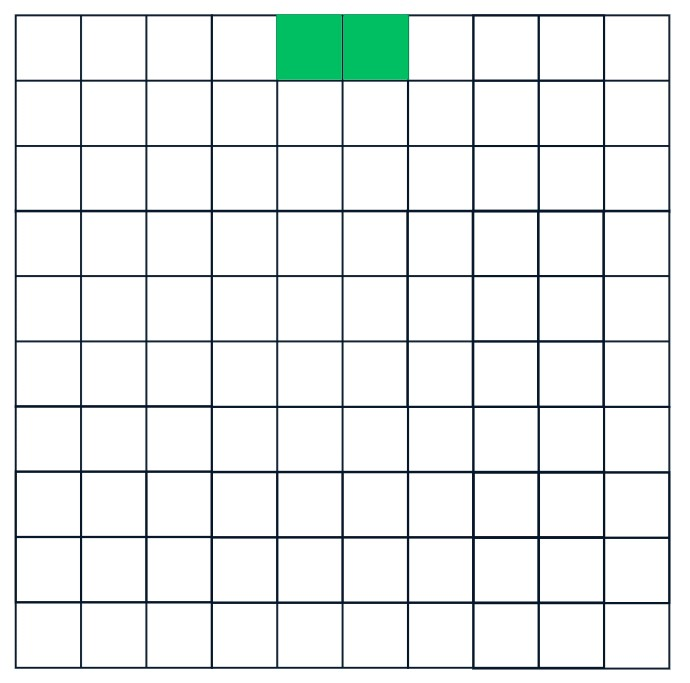
\includegraphics[scale=0.35]{gambar/gridkamera.jpg}
  % Ubah dengan keterangan gambar yang diinginkan
  \caption{Posisi Kursi Pada grid.}
  \label{fig:Posisi}
\end{figure}

Dapat dilihat posisi kursi roda mengambil 2 kotak grid hijau pada bagian (5,1) dan (6,1) dimana keputusan ini didasarkan lebar kursi roda yang sesuai dengan ukuran grid ada. Pemilihan posisi atas menentukan index mana yang merupakan bagian kiri maupun kanan dalam grid. Dengan posisi atas ditetapkan sebagai posisi konstan kursi roda dan hasil input citra yang didapatkan bersebrangan dengan hasil deteksi (mirror) maka index dapat diposisikan sebagai berikut:

\begin{figure}[H]
  \centering
  % Ubah dengan nama file gambar dan ukuran yang akan digunakan
  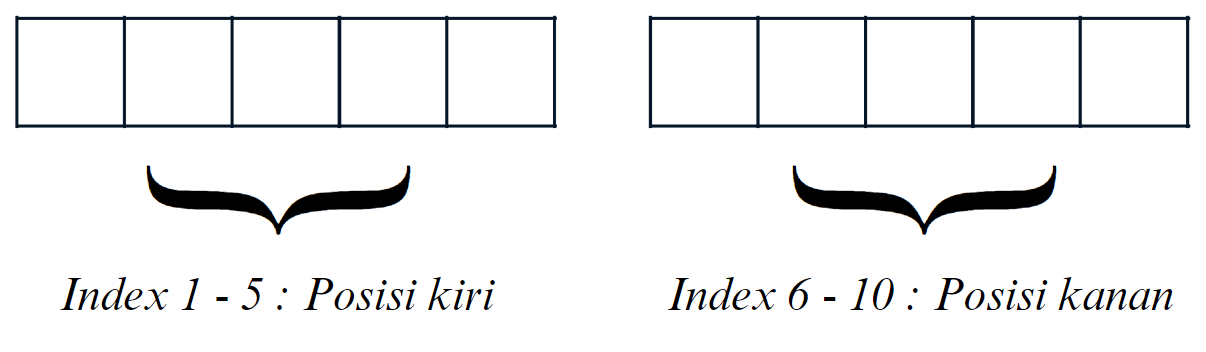
\includegraphics[scale=0.3]{gambar/posisi index sebenarnya.png}
  % Ubah dengan keterangan gambar yang diinginkan
  \caption{Kategori Posisi berdasarkan Index.}
  \label{fig:Kategori Posisi berdasarkan index.}
\end{figure}

Pengkategorian ini berperan penting dalam pengambilan keputusan belok kursi roda dimana nantinya hasil deteksi yang berupa jarak , lebar serta posisi relatif akan ditampilkan pada grid.

Secara horizontal posisi objek hasil deteksi akan diambil berdasarkan Nilai perpindahan titik X bounding box bawah relatif terhadap pixel. Yang mana nilainya akan disesuaikan dengan Resolusi frame yang didapatkan oleh kamera. Dimana akan dibuat patokan untuk posisi tertentu yang melambangkan perpindahan sebesar 0.2 meter secara horizontal.  Dengan asumsi bahwa kursi roda bergerak dan objek diam. maka hanya posisi objek yang terdeteksi didepanlah yang akan menjadi patokan penghindaran. Apabila objek terdeteksi namun saat berjalan maju objek menghilang maka kursi roda tidak perlu melakukan penghindaran. Oleh karena itu ditetapkan parameter jarak pada objek yang terdeteksi berdasarkan vertikal. Namun sebelum membahas lebih lanjut, akan dijelaskan secara rinci mengenai pemetaan hasil deteksi melalui hasil variabel yang didapat.

\begin{figure}[H]
  \centering
  % Ubah dengan nama file gambar dan ukuran yang akan digunakan
  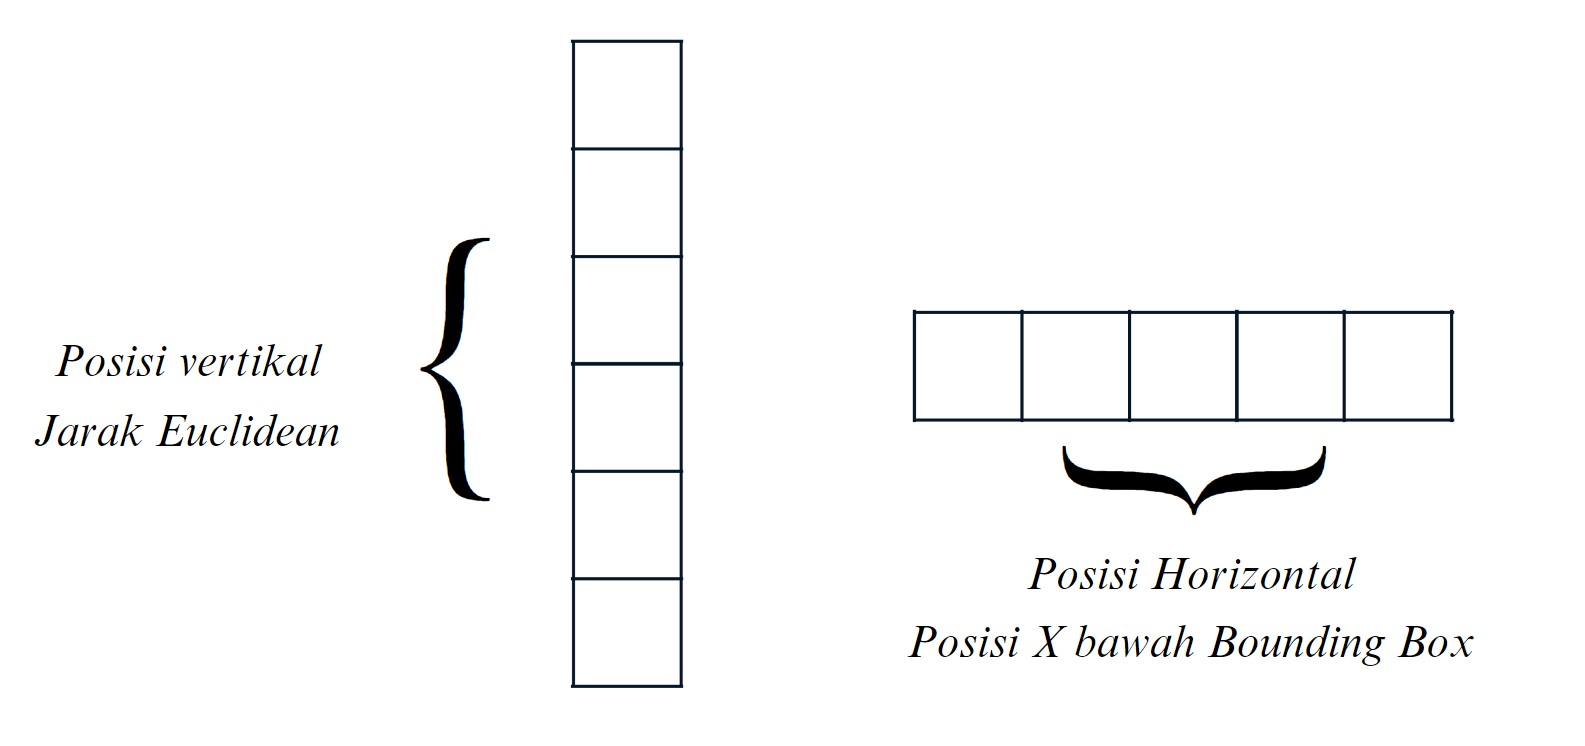
\includegraphics[scale=0.3]{gambar/posisi.jpg}
  % Ubah dengan keterangan gambar yang diinginkan
  \caption{Variabel Dalam perpindahan Posisi terhadap Grid.}
  \label{fig:Kategori Posisi berdasarkan index.}
\end{figure}

Berdasarkan Perhitungan rumus yang tadi didapatkan maka obstacle yang dideteksi dapat dipetakan posisinya relatif terhadap sumbu x dan y pada grid. Dimana keputusan mengambil variabel tersebut didasari oleh visibilitas hasil deteksi dan performa model dari hasil training. sehingga posisi yang dipetakan akan menjadi lebih akurat dan pengambilan keputusan dapat lebih konsisten. Namun dari posisi tersebut grid masih belum dapat merepresentasikan besar objek yang akan dilalui sehingga diperlukanlah sebuah variabel tambahan yang dapat membuat grid menggambar lebar objek relatif terhadap pixel yang nantinya akan dipetakan dalam grid. sehingga pada contoh gambar selanjutnya akan dijabarkan pemetaan lebar objek pada grid.

\begin{figure}[H]
  \centering
  % Ubah dengan nama file gambar dan ukuran yang akan digunakan
  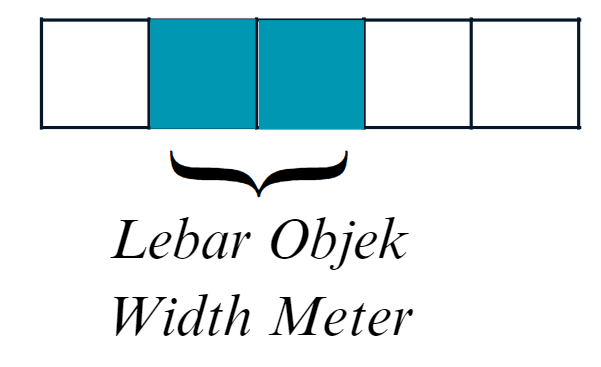
\includegraphics[scale=0.3]{gambar/Lebarobjek.png}
  % Ubah dengan keterangan gambar yang diinginkan
  \caption{Lebar Objek dalam grid.}
  \label{fig:Lebar Objek dalam grid.}
\end{figure}

Dapat dilihat pada gambar diatas pemetaan lebar berdasarkan nilai yang didapatkan pada variabel width meter. Dimana sesuai dengan parameter ukuran kotak yang telah ditentukan. Maka untuk setiap penambahan 0.2 meter ukuran lebar hasil deteksi yang didapatkan akan menambah jumlah kotak yang akan ditampilkan. 

Adapun beberapa kondisi dimana perlu dilakukannya kalibrasi mengingat bounding box yang ditampilkan tidak sepenuhnya dapat dengan akurat merepresentasikan posisi objek dalam horizontal sehingga perlunya ditambahkan sebuah nilai kalibrasi yang akan berperan dalam mengatasi limitasi bounding box yang kadang memiliki nilai tengah yang tidak konsisten. Penambahan nilai pada rumus dibawah dapat menyesuaikan nilai posisi x pada grid agar lebih mendekati nilai kenyataan.

\begin{equation}
    Grid\_x = (\frac{posisi\_x\_bounding\_box +konstanta}{scale\_factor})
\end{equation}

Setelah pemetaan grid dilakukan selanjutnya akan ditampilkan parameter yang akan digunakan dalam pengambilan keputusan belok kursi roda.

\subsection{Output Hasil deteksi}
Dalam menentukan keputusan dalam pembelokan kursi roda akan ditambahkan beberapa parameter. Parameter ini berfungsi untuk menentukan Kapan kursi roda harus berbelok dan seberapa jauh kursi roda harus berbelok. Parameter tersebut akan dibagi menjadi beberapa status yang dimana kondisi-kondisi yang telah ditetapkan harus terpenuhi untuk dapat dikatakan memenuhi syarat.

\subsubsection*{1. Valid Object Condition}
Pada kondisi ini objek harus terdeteksi pada input citra untuk memenuhi kondisi ini. Tidak ada parameter khusus yang mengharuskan kursi roda untuk berbelok dalam kondisi ini, karena posisi kursi roda masih tergolong jauh dari posisi hasil deteksi. Dimana pengambilan keputusan yang akan dilakukan kursi roda adalah untuk tetap maju. Berikut merupakan contoh gambar untuk kondisi yang memenuhi. 

\begin{figure}[H]
  \centering
  % Ubah dengan nama file gambar dan ukuran yang akan digunakan
  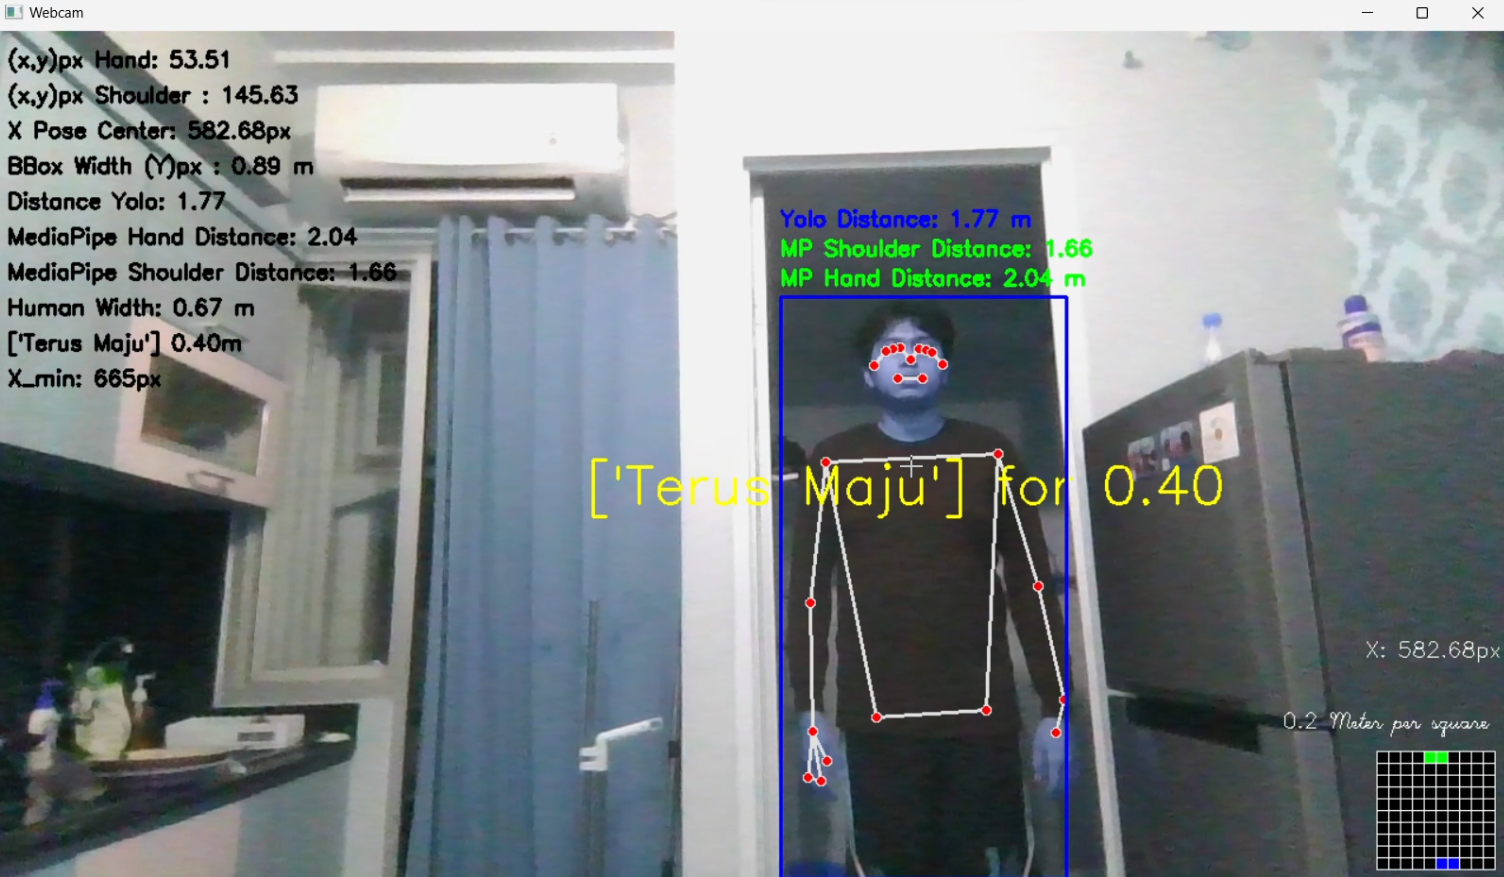
\includegraphics[scale=0.3]{gambar/posisibiru.png}
  % Ubah dengan keterangan gambar yang diinginkan
  \caption{Contoh valid object diatas 0.8 Meter.}
  \label{fig:Valid object diatas 0.8 Meter.}
\end{figure}

Dapat dilihat pada gambar diatas dimana objek hanya terdeteksi namun belum terdapat indikasi mendesak untuk kursi roda dalam mengambil keputusan karena posisi hasil deteksi yang masih tergolong jauh. adapun warna bounding box yang digambar berwarna biru sebagai penanda objek tergolong \emph{safe distance} terhadap kursi roda. Sehingga instruksi yang akan dikirim adalah tetap maju. 

\begin{figure}[H]
  \centering
  % Ubah dengan nama file gambar dan ukuran yang akan digunakan
  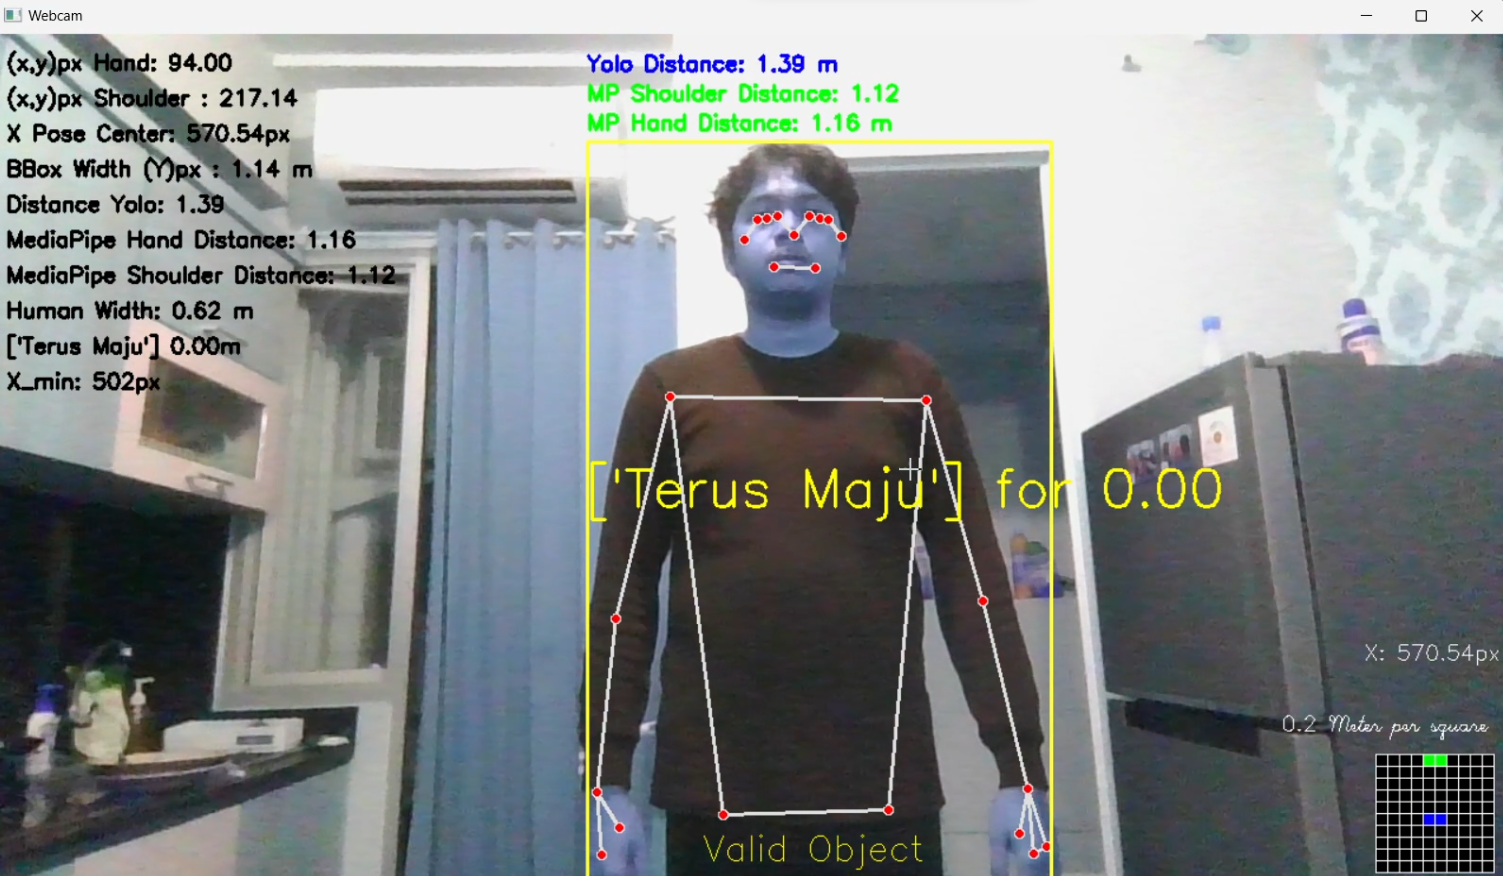
\includegraphics[scale=0.3]{gambar/posisikuning.png}
  % Ubah dengan keterangan gambar yang diinginkan
  \caption{Contoh valid object dibawah 0.8 Meter.}
  \label{fig:Valid object diatas 0.8 Meter.}
\end{figure}

Saat hasil objek yang terdeteksi menjadi lebih dekat terhadap kursi roda maka bounding box akan berubah menjadi warna kuning yang menjadi indikasi bahwa objek yang terdeteksi sudah dibawah 0.8 Meter. sejauh ini pengambilan keputusan untuk belok belum dilakukan, namun akan menampilkan "valid object" pada bagian bawah layar kamera. Mengindikasikan objek benar-benar terdeteksi dan mulai mendekati. Dapat dilihat juga pada Grid di pojok kanan bawah bahwa perpindahan telah terjadi yang direpresentasikan berdasarkan perhitungan variabel yang ditampilkan pada pojok kanan atas layar kamera. Adapun beberapa contoh lainnya dapat dilihat digambar berikut.

\begin{figure}[H]
  \centering
  % Ubah dengan nama file gambar dan ukuran yang akan digunakan
  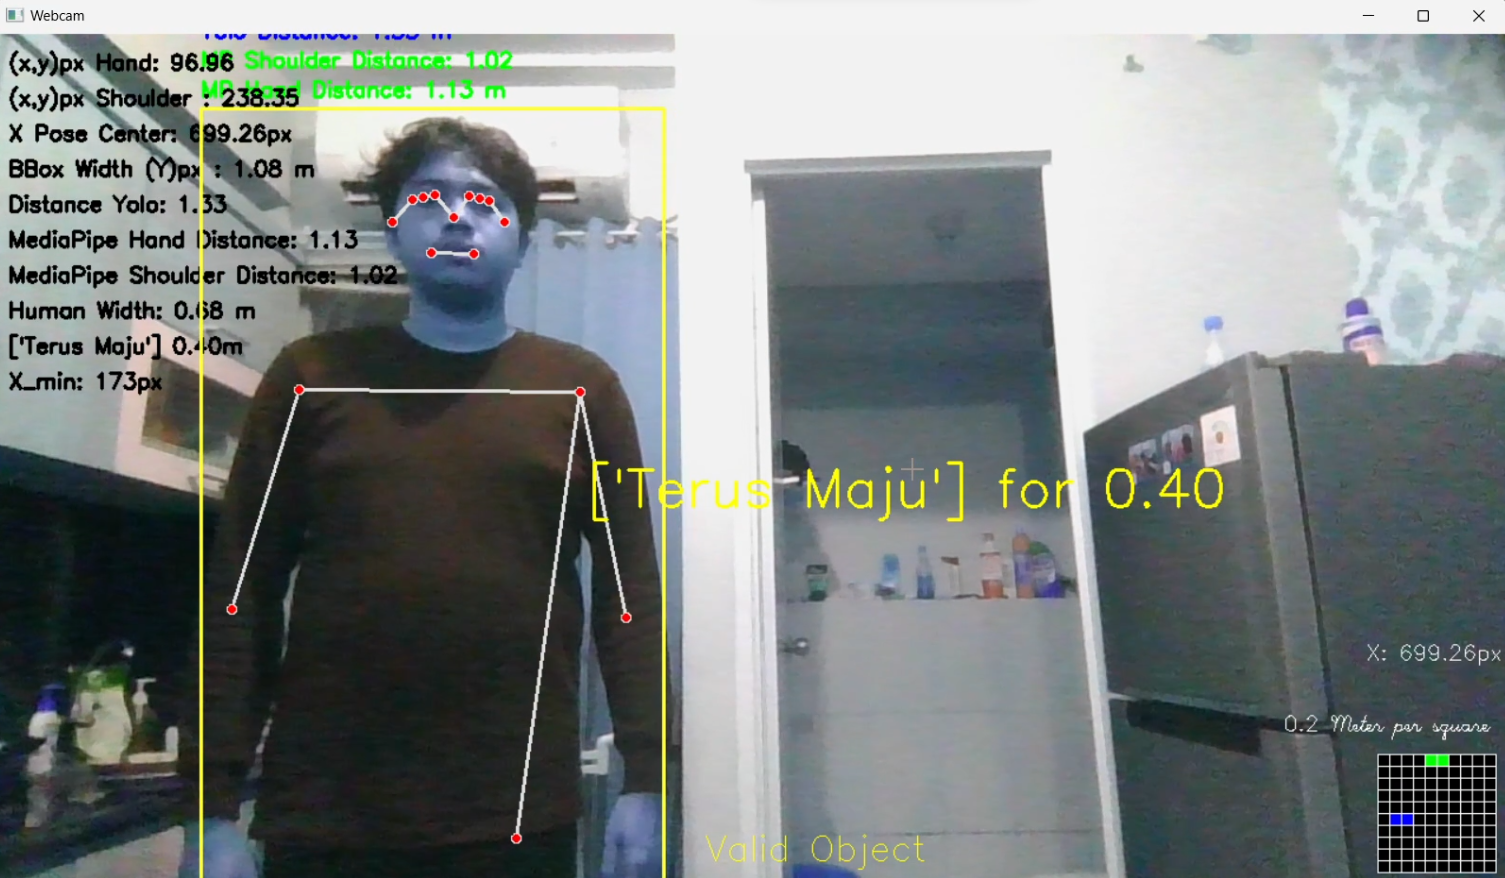
\includegraphics[scale=0.3]{gambar/posisikuning kiri.png}
  % Ubah dengan keterangan gambar yang diinginkan
  \caption{Contoh lain valid object dibawah 0.8 Meter condong kiri.}
  \label{fig:Contoh lain Valid object dibawah 0.8 Meter.}
\end{figure}

\begin{figure}[H]
  \centering
  % Ubah dengan nama file gambar dan ukuran yang akan digunakan
  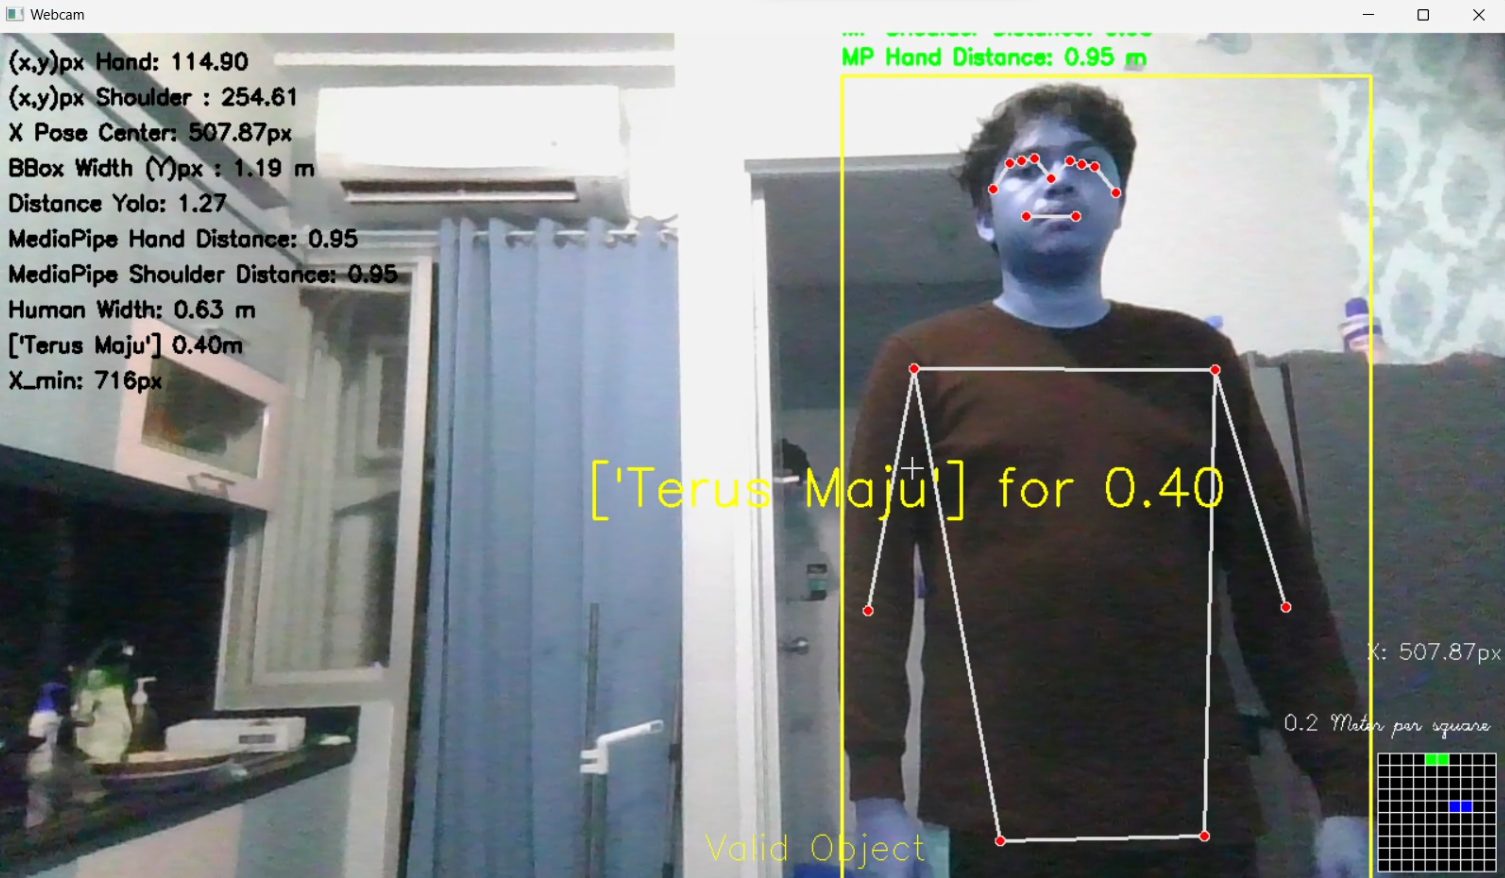
\includegraphics[scale=0.3]{gambar/posisikuning kanan.png}
  % Ubah dengan keterangan gambar yang diinginkan
  \caption{Contoh lain valid object dibawah 0.8 Meter condong kanan.}
  \label{fig:Valid object dibawah 0.8 Meter.}
\end{figure}

\subsubsection{2. Near Object Condition}
Pada kondisi ini objek harus terdeteksi pada input citra untuk memenuhi kondisi ini dan objek harus berada dibawah 0.5 Meter jarak terdeteksi. Dalam kondisi ini akan dibagi menjadi 3 pengambilan keputusan. yaitu sebagai berikut: 

\subsubsection*{Hasil deteksi objek pada grid menunjukan Index Kiri Lebih besar dari Index kanan}
Pada kondisi ini posisi hasil deteksi menunjukan nilai yang lebih besar pada Index kiri (Index 1-5) yang berarti bahwa objek sedang berada pada sebelah kiri posisi terhadap kursi roda. Dapat dilihat pada contoh gambar dibawah.

\begin{figure}[H]
  \centering
  % Ubah dengan nama file gambar dan ukuran yang akan digunakan
  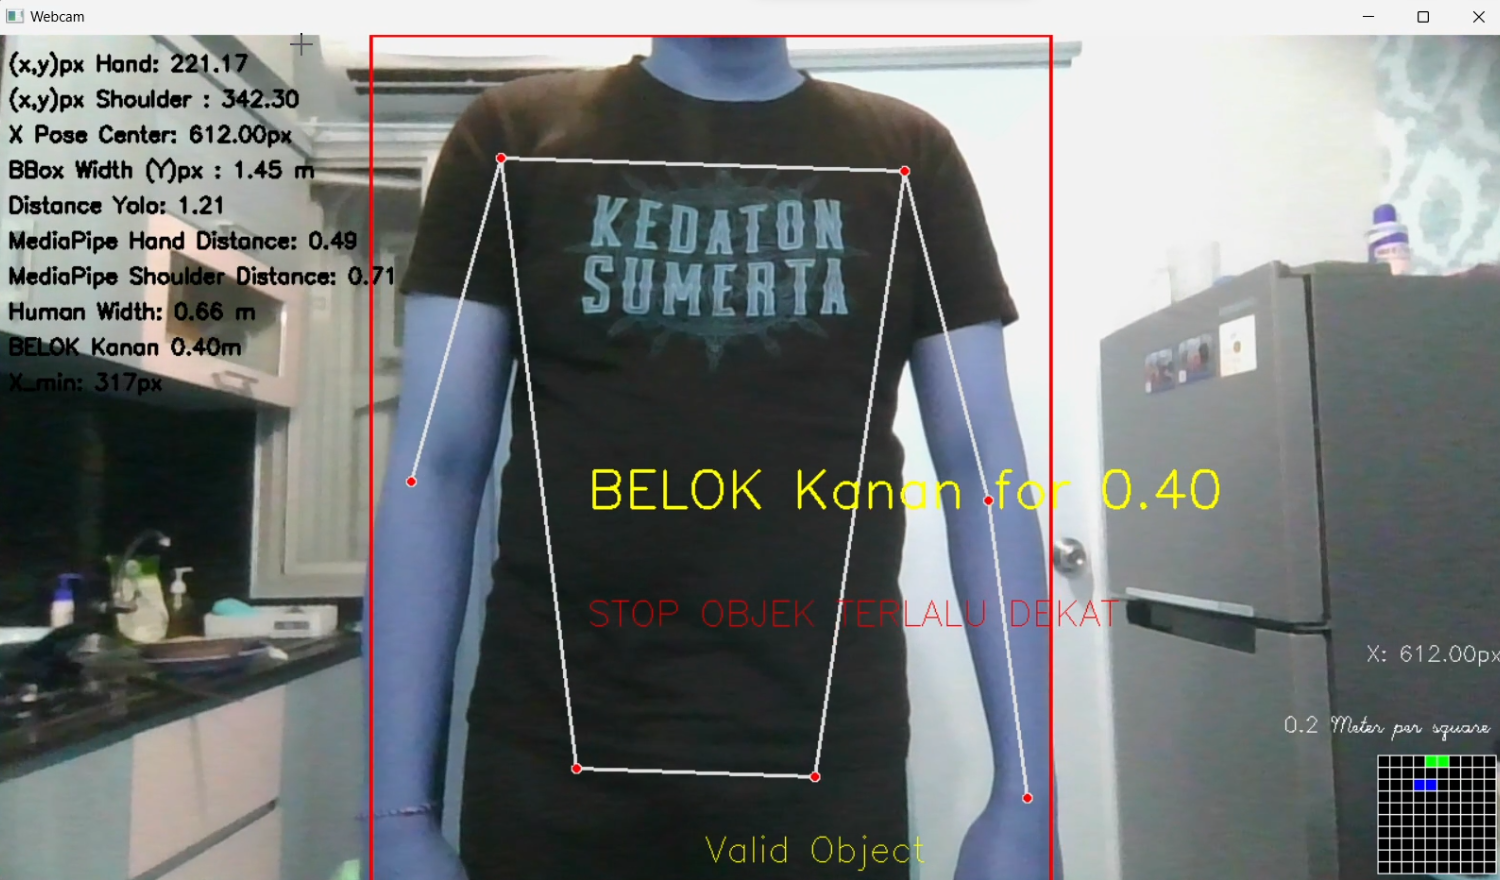
\includegraphics[scale=0.3]{gambar/merahkiri.png}
  % Ubah dengan keterangan gambar yang diinginkan
  \caption{Contoh kondisi Near Object Index Kiri \textgreater Kanan .}
  \label{fig:Valid object dibawah 0.8 Meter.}
\end{figure}

Dapat dilihat pada gambar, grid nilainya lebih mengarah index kiri dari pada kanan. Dimana dilihat dari pertimbangan posisi tersebut maka kursi roda akan menghindar ke Kanan yang merupakan belokan yang lebih aman ketimbang belokan ke kiri.

\subsubsection*{Hasil deteksi objek pada grid menunjukan index Kanan lebih besar dari Index kiri}
Pada kondisi ini posisi hasil deteksi menunjukan nilai yang lebih besar pada index kanan (6-10) yang berarti bahwa objek sedang berada pada sebelah kanan posisi terhadap kursi roda. dapat dilihat pada contoh gambar dibawah

\begin{figure}[H]
    \centering
    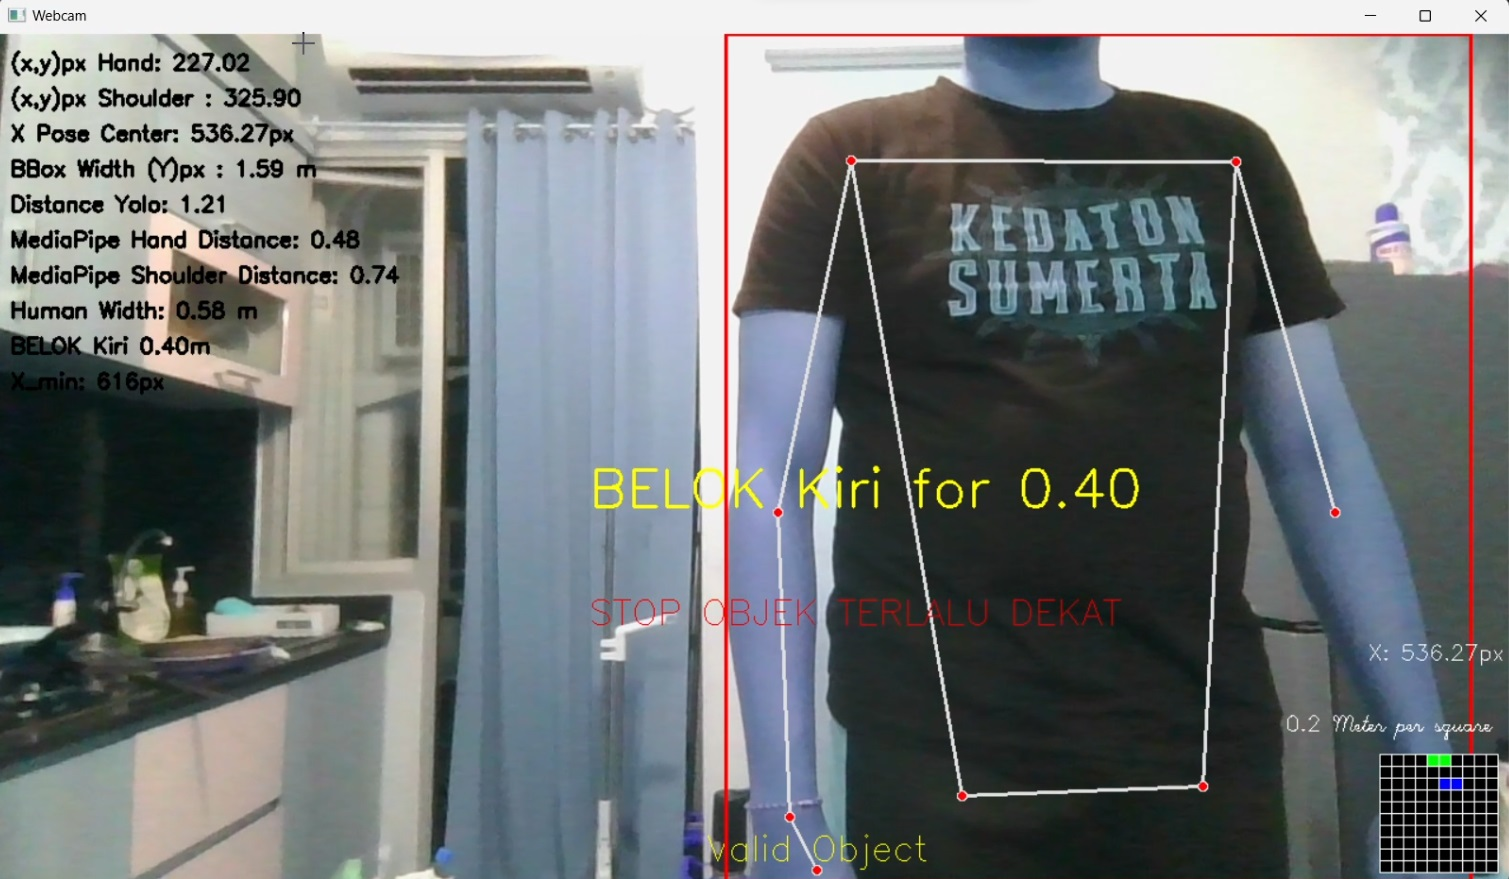
\includegraphics[scale=0.3]{gambar/merahkanan.jpg}
    \caption{Contoh kondisi Near Object Index Kanan \textgreater kiri}
    \label{fig:Near Object index kanan>kiri}
\end{figure}

Dapat dilihat pada gambar, grid nilainya lebih mengarah index kanan dari pada kiri. Dimana dilihat dari pertimbangan posisi tersebut maka kursi roda akan menghindar ke kiri yang merupakan belokan yang lebih aman ketimbang belokan ke kanan.

\subsubsection*{Hasil deteksi objek pada grid menunjukan posisi Linear terhadap kursi roda}
Pada kondisi ini perlu ditambahkan sebuah perintah untuk pengambilan keputusan dimana posisi belok pada kondisi ini baik melalui kanan maupun kiri tidak akan memiliki kelebihan/kekurangan karena dalam posisi ini nilai index sama besarnya baik kanan maupun kiri. sehingga perlu dilakukan pendekatan yang baik agar pengambilan keputusan ini tidak menimbulkan kesalahan. Pada tugas proyek ini pengambilan keputusan ini didasari pada nilai random. Sehingga keputusan yang diambil bisa ke kanan maupun ke kiri. 

\begin{figure}[H]
    \centering
    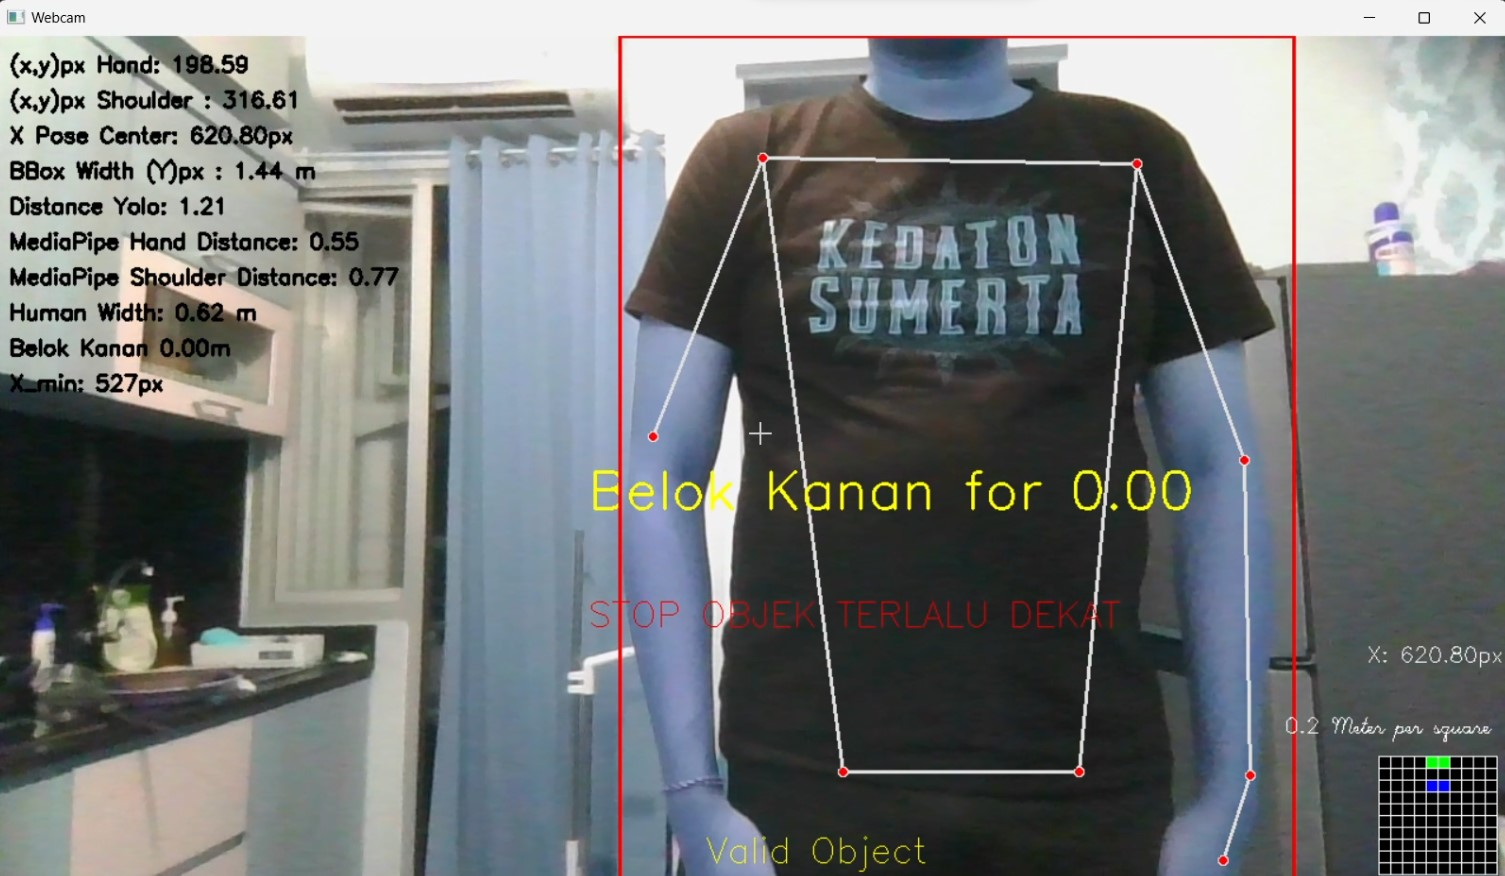
\includegraphics[scale=0.3]{gambar/merahlinier.jpg}
    \caption{Contoh kondisi Near Object Liniear.}
    \label{fig:Near Object Linear}
\end{figure}

Dapat dilihat pada gambar, gridnya sejajar dengan posisi kursi roda. Sehingga penggunaan random akan sangat berguna untuk mengabil keputusan apabila menghadapi kasus seperti ini.

